
\section{Élaboration du modèle de connaissance d'un actionneur linéaire placé sur un banc d'essai}% III
%III.A - 
\subsection{Étude de la dynamique de l'actionneur linéaire dans le cas particulier représentatif de la mise en précontrainte étudiée à la question \ref{ccs_mp_2023_q_03} modélisant le système dans cette configuration particulière}

\begin{obj}
Définir un modèle de connaissance de la dynamique du système permettant d'obtenir les équations d'un modèle de simulation comparable aux mesures du banc d'essai.
\end{obj}

\ifprof
\else

Le système est placé sur un banc d'essai en position horizontale (figure \ref{ccs_mp_2023_fig_08}). Dans cette configuration, la pesanteur est portée par la direction $\vec{z}_{0}$. On rappelle que le banc fonctionne selon deux protocoles distincts

\begin{itemize}
  \item vérification de la course définie précédemment (non étudiée ici) ;
  \item vérification de la force exercée par un actionneur linéaire pour effectuer la précontrainte.
\end{itemize}

%\begin{figure}[h]
%\begin{center}
%  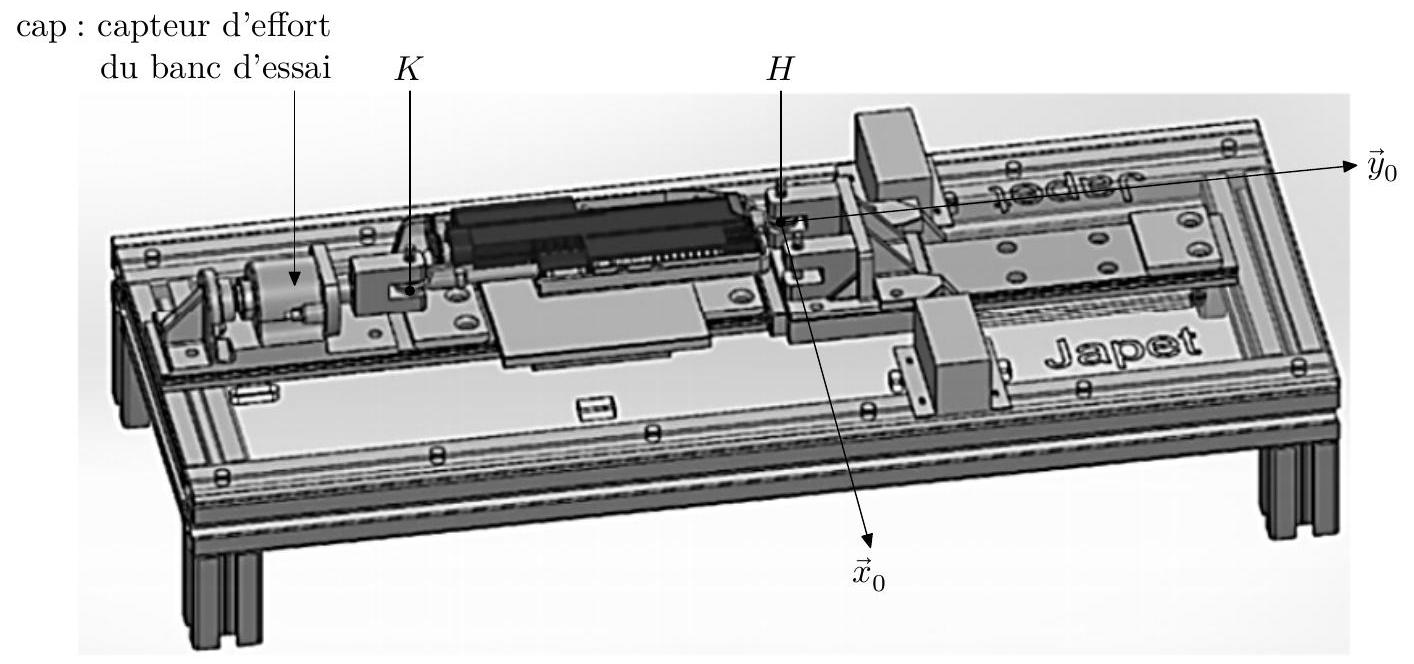
\includegraphics[width=\textwidth]{2025_09_16_5f2d7643f7e649c6833dg-06(1)}
%\captionsetup{labelformat=empty}
%\caption{Figure 8 Banc d'essai}
%\end{center}
%\end{figure}


\begin{figure}[!h]
\centering
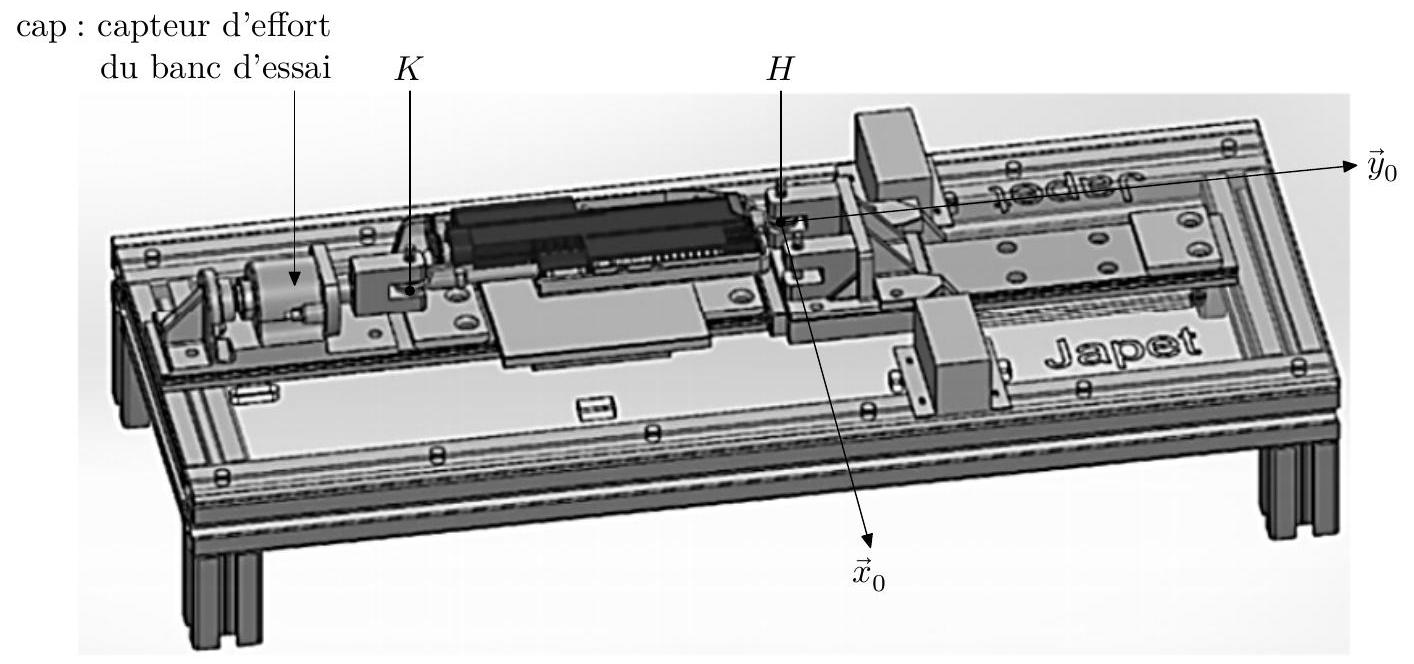
\includegraphics[width=.8\textwidth]{2025_09_16_5f2d7643f7e649c6833dg-06(1)}
\caption{\label{ccs_mp_2023_fig_08}  Banc d'essai}
\end{figure}



Pour la vérification de la force de précontrainte, l'actionneur linéaire est bloqué en $H$ et un capteur d'effort, noté cap (figure \ref{ccs_mp_2023_fig_08}), supposé indéformable, est placé en $K$. Cette configuration permet uniquement de valider la performance relative à la mise en précontrainte.\\
La raideur du ressort du capteur d'effort de l'actionneur linéaire (figure \ref{ccs_mp_2023_fig_09}) a été choisie à partir d'une campagne d'essais réalisée par différents utilisateurs qui ont exprimé leur ressenti en donnant une note de confort. L'exploitation des données recueillies a permis au fabricant de déterminer le meilleur compromis parmi les retours des différents utilisateurs.

Chaine d'action : transmission de l'énergie par une chaine moteur-réducteur-vis-écrou

%\begin{figure}[h]
%\begin{center}
%  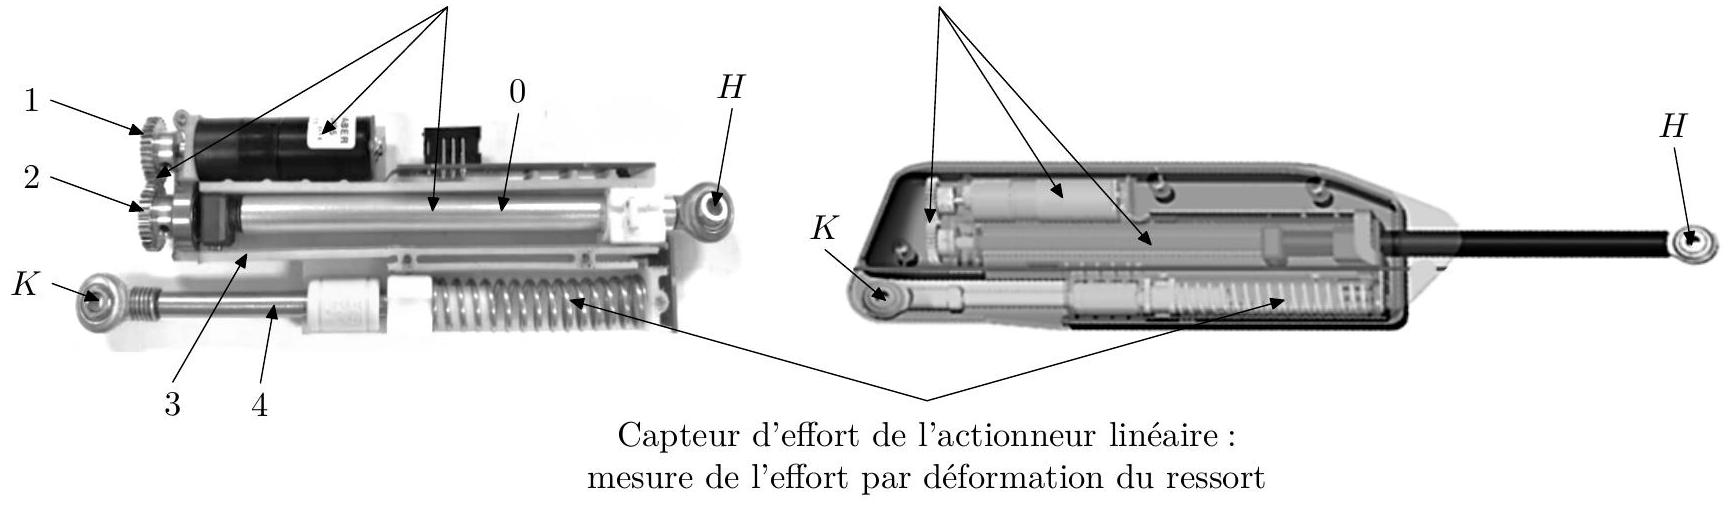
\includegraphics[width=\textwidth]{2025_09_16_5f2d7643f7e649c6833dg-06}
%\captionsetup{labelformat=empty}
%\caption{Figure 9 Actionneur linéaire}
%\end{center}
%\end{figure}


\begin{figure}[!h]
\centering
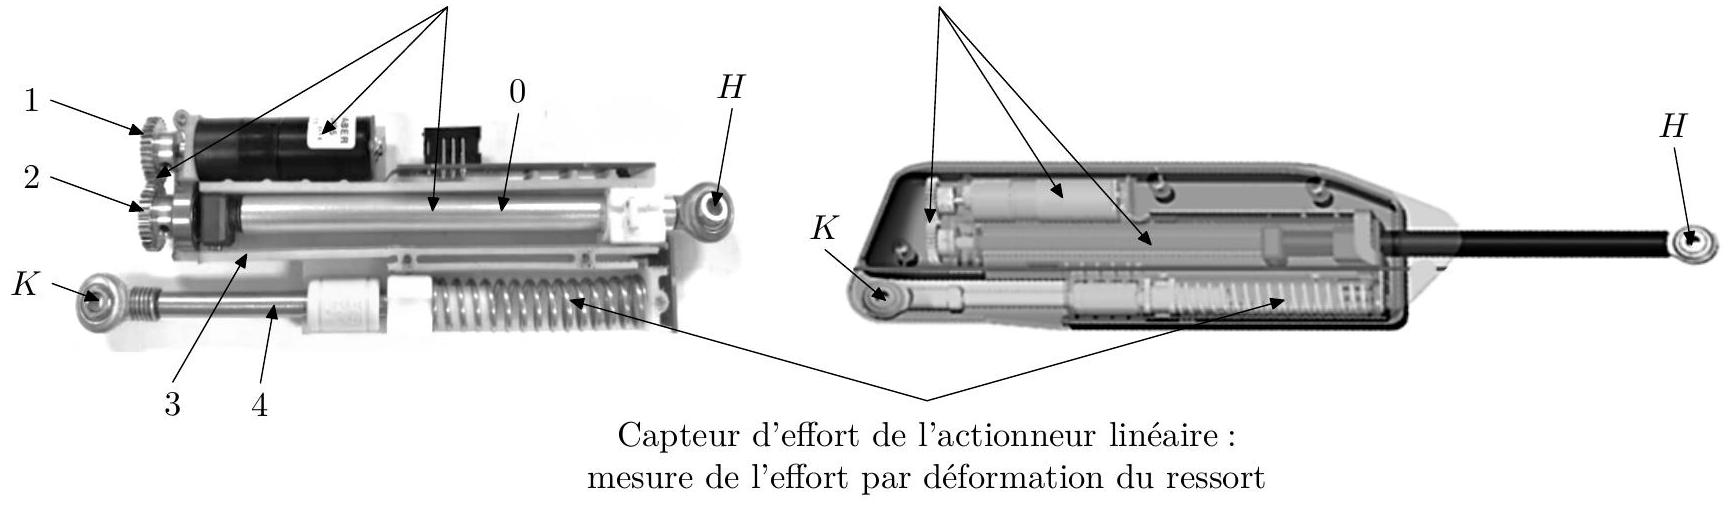
\includegraphics[width=\textwidth]{2025_09_16_5f2d7643f7e649c6833dg-06}
\caption{\label{ccs_mp_2023_fig_09} Actionneur linéaire }
\end{figure}


Dans la configuration spécifique retenue, les points $K$ et $H$ sont immobiles par rapport au châssis du banc d'essai. Les solides (0) et (4) sont immobiles par rapport au châssis du banc d'essai. L'action mécanique de l'actionneur linéaire sur le capteur d'effort du banc d'essai est un glisseur de support passant par $K$ et de résultante $\vec{F}_{4 \rightarrow \text { cap }}$. Le capteur du banc d'essai mesure ainsi $\vec{F}_{4 \rightarrow \text { cap }} \cdot \vec{y}_{0}$. On suppose que c'est une image fidèle de la force de traction exercée par l'actionneur linéaire.

%\begin{figure}[h]
%\begin{center}
%  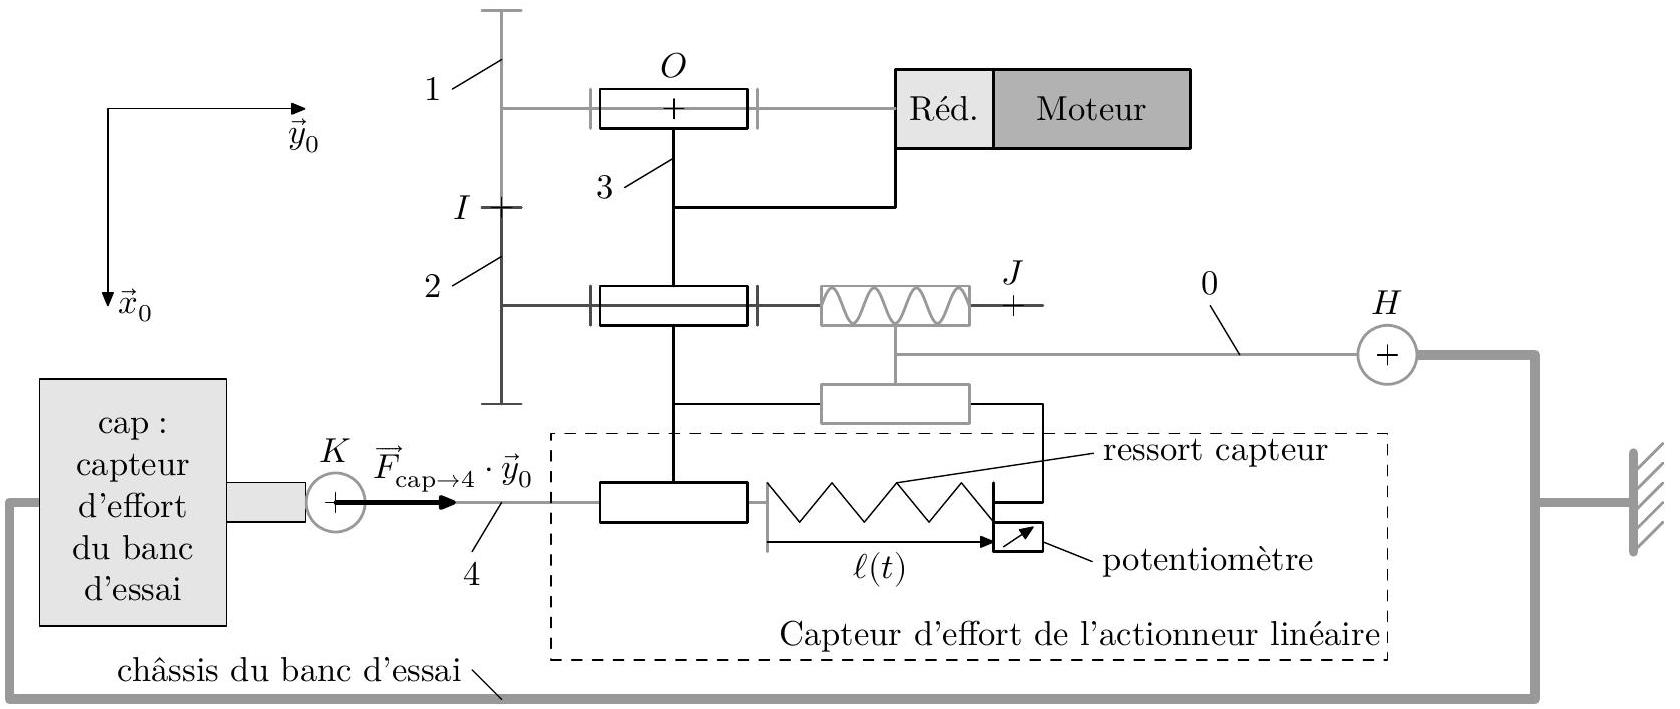
\includegraphics[width=\textwidth]{2025_09_16_5f2d7643f7e649c6833dg-07}
%\captionsetup{labelformat=empty}
%\caption{Figure 10 Modèle d'étude de l'actionneur linéaire sur le banc d'essai}
%\end{center}
%\end{figure}


\begin{figure}[!h]
\centering
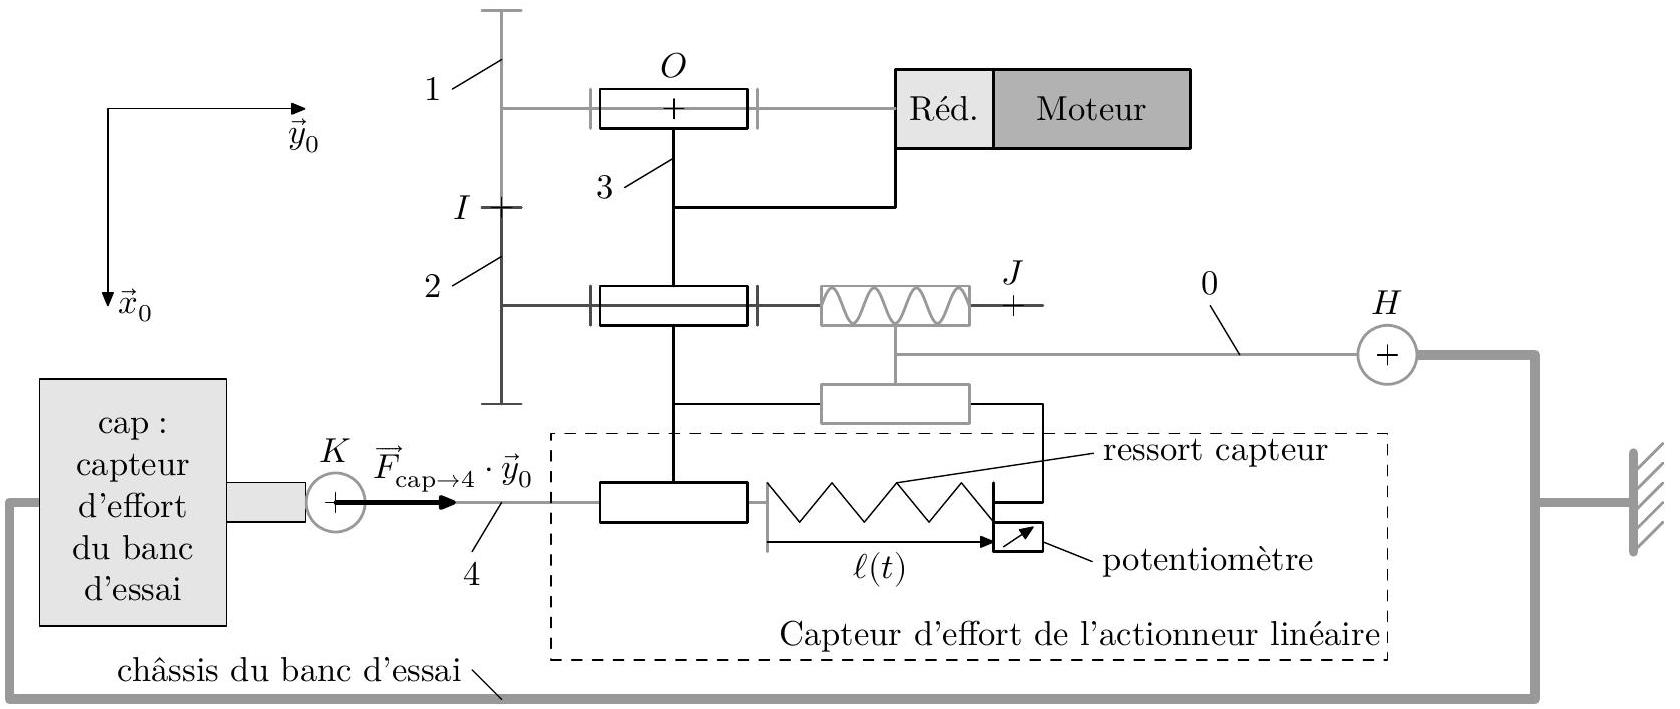
\includegraphics[width=.9\textwidth]{2025_09_16_5f2d7643f7e649c6833dg-07}
\caption{\label{ccs_mp_2023_fig_10}  Modèle d'étude de l'actionneur linéaire sur le banc d'essai}
\end{figure}



On note $\ell(t)$ le déplacement de (3) par rapport à (4).

On a $y(t)=\ell_{0}-\ell(t)$ avec $\ell_{0}$ la longueur à vide du ressort du capteur installé sur le système réel. Le ressort n'est pas préchargé avant le début de l'essai soit $\ell(t=0)=\ell_{0}$.

Le repère $R_{0}\left(H ; \vec{x}_{0}, \vec{y}_{0}, \vec{z}_{0}\right)$ lié au châssis du banc d'essai est supposé galiléen.

Les différentes grandeurs utiles à cette partie sont regroupées dans le tableau \ref{ccs_mp_2023_tab_03}.

\begin{table}[!h]
\begin{center}
\begin{tabular}{lp{8cm}}
\hline
\textbf{Éléments} & \textbf{Caractéristiques et notation} \\
\hline
Corps du vérin 0 & Masse : $m_{0}$ \\
\hline
\multirow[t]{4}{*}{Moteur} & Couple moteur : $C_{3 \rightarrow \text { arbre moteur }}(t)=c_{m}(t)$ \\

 & Moment d'inertie de l'arbre moteur suivant son axe : $I_{m}$ \\

 & Vitesse de rotation de l'arbre moteur : $\omega_{m}(t)=\omega_{m / 3}$ \\

 & Masse négligeable devant les autres masses \\
\hline
\multirow[t]{4}{*}{Réducteur planétaire + pignon 1} & Vitesse de rotation en sortie du réducteur : $\omega_{r}(t)=\omega_{1 / 3}$ \\

 & Rapport de réduction : $\lambda=\frac{\omega_{r}(t)}{\omega_{m}(t)}$ \\

 & Moment d'inertie équivalent reporté sur l'arbre de sortie du réducteur : $I_{r}$ \\

 & Masse négligeable devant les autres masses \\
\hline
\multirow[t]{2}{*}{Transmetteur par engrenage} & Nombre de dents du pignon d'entrée 1: $Z_{1}$ \\

 & Nombre de dents du pignon de sortie 2 : $Z_{2}=Z_{1}$ \\
\hline
\multirow[t]{3}{*}{Vis + pignon 2} & Moment d'inertie suivant l'axe ( $J, \vec{y}_{0}$ ) : $I_{V}$ \\

 & Vis de pas géométrique : pas en $\mathrm{m} \cdot \operatorname{tr}^{-1}$ \\

 & Masse négligeable devant les autres masses \\
\hline
\multirow[t]{2}{*}{Ressort} & Raideur $K_{\text {res }}$ \\

 & Masse négligeable devant les autres masses \\
\hline
Ensemble 3 & Masse $m_{3}$ (les masses du carter moteur et du carter réducteur sont comprises dans la masse $m_{3}$ ) \\
\hline
Tige de vérin 4 & Masse : $m_{4}$ \\
\hline
Rendement & Rendement global de l'actionneur linéaire, supposé constant : $\eta$ \\
\hline
\end{tabular}
%\captionsetup{labelformat=empty}
\caption{\label{ccs_mp_2023_tab_03} Caractéristiques principales de l'actionneur linéaire}
\end{center}
\end{table}
\fi


%Q 5. 
\question{\label{ccs_mp_2023_q_05}
En prenant soin de préciser le solide isolé et le théorème utilisé, déterminer l'expression littérale de la résultante $\vec{F}_{\text {cap } \rightarrow 4}$ en projection sur $\vec{y}_{0}$, en fonction de $K_{\text {res }}$ et $y(t)$.}
\ifprof
\begin{corrige}
\begin{itemize}
On isole le solide 4.
\item BAME -- 4 est soumis à :
\begin{itemize}
\item l'action mécanique transmise par la liaison glissière entre 3 et 4 d'axe $\overrightarrow{y}_0$;
\item l'action du capteur $\overrightarrow{F}_{\text{cap} \to 4}$;
\item l'effort de rappel du ressort $-K_{\text{res}} y(t) \overrightarrow{y}_0$.
\end{itemize}
\end{itemize}

Le Théorème de la Résultante Statique (solide (4) immobile) projetée selon $\overrightarrow{y}_0$ donne:

$$ \boxed{0 = \overrightarrow{F}_{\text{cap} \to 4} \cdot \overrightarrow{y}_0 - K_{\text{res}} y(t)} $$

\end{corrige}
\else
\fi

%Q 6. 
\question{\label{ccs_mp_2023_q_06}
Déterminer le rapport $\frac{\omega_{1 / 3}}{\omega_{2 / 3}}$ en fonction de $Z_{1}$ et $Z_{2}$ et faire l'application numérique. En déduire l'expression de $\vec{V}_{J, 3 / R_{0}}$ en fonction de $\omega_{m}(t)$, pas et $\lambda$.\\
}
\ifprof
\begin{corrige}
On a un système pignon + roue dentée à axes fixes, donc: $\boxed{\dfrac{\omega_{1/3}}{\omega_{2/3}} = - \dfrac{Z_2}{Z_1} = -1}$.\\

Par composition des vitesses: $\overrightarrow{V}_{J,3/R_0} = \overrightarrow{V}_{J,3/2} + \overrightarrow{V}_{J,2/R_0}$, or $\overrightarrow{V}_{J,3/2} = \overrightarrow{0}$ car $J$ est situé sur l'axe de rotation de la liaison pivot entre (3) et (2). De plus $\overrightarrow{V}_{J,2/R_0} = \dfrac{pas}{2\pi} \omega_{2/R_0}\overrightarrow{y}_0$.\\

Encore par composition des vitesses $\omega_{2/R_0} = \omega_{2/3} + \omega_{3/R_0}$ et $\omega_{3/R_0} = 0$ par la liaison glissière entre (3) et (0). De plus $\omega_{2/3} = -\omega_{1/3} = - \lambda \omega_m(t)$.\\

Pour conclure $\boxed{\overrightarrow{V}_{J,3/R_0} = - \dfrac{pas}{2\pi} \lambda \omega_m(t) \overrightarrow{y}_0}$.

\end{corrige}
\else
\fi

On note $\Sigma=\left\{(0)\right.$, arbre moteur, (1), (2), (3), ressort, (4)\} l'ensemble mobile en mouvement par rapport à $R_{0}$.\\

%%Q 7. 
%\question{\label{ccs_mp_2023_q_07}
%Déterminer l'expression des énergies cinétiques $E_{c}\left(\right.$ arbre moteur $\left./ R_{0}\right), E_{c}\left(1 / R_{0}\right), E_{c}\left(2 / R_{0}\right)$ et $E_{c}\left(3 / R_{0}\right)$ en fonction de $\omega_{m}(t)$, pas, $\lambda$, de la masse $m_{3}$ et des inerties.}
%\ifprof
%\begin{corrige}
%
%\end{corrige}
%\else
%\fi
%
%
%%Q 8. \\
%\question{\label{ccs_mp_2023_q_08}
%Écrire l'expression de l'énergie cinétique $E_{c}\left(\Sigma / R_{0}\right)$ et en déduire l'expression du moment d'inertie équivalent $I_{\text {eq }}$ de l'ensemble mobile $\Sigma$ reporté sur l'arbre moteur en fonction de pas, $\lambda$, de la masse $m_{3}$ et des inerties.}
%\ifprof
%\begin{corrige}
%\end{corrige}
%\else
%\fi
%
%
%%Q 9. \\
%\question{\label{ccs_mp_2023_q_09}
%Établir le bilan des puissances galiléennes des actions extérieures s'exerçant sur $\Sigma$ et montrer qu'elles sont toutes nulles.}
%\ifprof
%\begin{corrige}
%\end{corrige}
%\else
%\fi
%
%
%%Q 10. \\
%\question{\label{ccs_mp_2023_q_10}
%Établir le bilan des puissances des actions intérieures à $\Sigma$ et déterminer leurs expressions littérales en justifiant les résultats.}
%\ifprof
%\begin{corrige}
%\end{corrige}
%\else
%\fi
%
%
%%Q 11. 
%\question{\label{ccs_mp_2023_q_11}
%Par composition des vecteurs vitesse en $K$ entre les solides (4), (3) et (0), déterminer la relation entre $\dot{y}(t), \omega_{m}(t)$, pas et $\lambda$.}
%\ifprof
%\begin{corrige}
%\end{corrige}
%\else
%\fi
%
%
%Pour la suite, on définit $K_{\text {trans }}$ tel que $\dot{y}(t)=K_{\text {trans }} \cdot \omega_{m}(t)$.\\
%
%%Q 12. 
%\question{\label{ccs_mp_2023_q_12}
%En appliquant le théorème de l'énergie cinétique à l'ensemble $\Sigma$ en mouvement par rapport à $R_{0}$, montrer que l'équation de mouvement s'écrit sous la forme 
%$
%I_{\mathrm{eq}} \frac{\mathrm{~d} \omega_{m}(t)}{\mathrm{d} t}=Q c_{m}(t)-c_{r}(t) \quad \text { avec } \quad c_{r}(t)=T y(t)
%$
%où l'on précisera les expressions de $Q$ et $T$ en fonction de $\eta, K_{\text {res }}$ et $K_{\text {trans }}$.\\}
%\ifprof
%\begin{corrige}
%\end{corrige}
%\else
%\fi
%
%
%%Q 13. \\
%\question{\label{ccs_mp_2023_q_13}
%Exprimer l'équation différentielle du mouvement liant le déplacement $y(t)$ à l'action mécanique $c_{m}(t)$ en fonction des paramètres de $Q, T$ et $K_{\text {trans }}$. En déduire la valeur numérique du facteur d'amortissement et conclure quant à l'amortissement de la réponse indicielle.}
%\ifprof
%\begin{corrige}
%\end{corrige}
%\else
%\fi
%
%Cet ensemble d'équations permet de mettre en place un modèle de connaissance de l'actionneur linéaire placé sur le banc d'essai et son analyse justifie la mise en place d'une structure particulière de l'asservissement.

\subsection{Étude de l'effort d'assistance nécessaire au soutien lombaire}%III.B - 
%\section{Objectif}
\begin{obj}
Proposer un modèle de connaissance de l'asservissement en force, le valider par comparaison avec une mesure sur un banc d'essai et vérifier les performances de l'actionneur linéaire sur un banc d'essai. Ce modèle permettra de valider une commande pour le cas spécifique étudié.
\end{obj}


%\section{III.B.1) Mise en place d'un modèle de connaissance}
\subsubsection{Mise en place d'un modèle de connaissance}%III.B.1) 
\ifprof
\else

L'actionneur linéaire placé sur le banc d'essai et sa commande peuvent être modélisés par le schéma-blocs représenté figure \ref{ccs_mp_2023_fig_11}.\\
Notations et hypothèses:

\begin{itemize}
  \item la transformée de Laplace de la fonction $a(t)$ est notée $A(p)$ dans le cas général ;
  \item les conditions de Heaviside sont supposées vérifiées;
  \item $F_{c}(p)$ représente la consigne en force de l'asservissement de force, dans le domaine de Laplace;
  \item $F(p)$ représente la force développée par l'actionneur linéaire, dans le domaine de Laplace.
\end{itemize}

Les équations modélisant le comportement du moteur électrique (moteur à courant continu) muni d'une boucle d'asservissement de l'intensité du courant $i_{m}(t)$, sont :

\begin{itemize}
  \item en supposant le temps de réponse de la boucle de courant négligeable,
\end{itemize}

$$
u_{I}(t)=R i_{m}(t)
$$

\begin{itemize}
  \item par application des théorèmes généraux de la dynamique appliqués à l'ensemble des solides en mouvement,
\end{itemize}

$$
I_{\mathrm{eq}} \frac{\mathrm{~d} \omega_{m}(t)}{\mathrm{d} t}=Q c_{m}(t)-c_{r}(t) \quad \text { avec } \quad c_{r}(t)=T y(t)
$$

\begin{itemize}
  \item loi de couplage électromécanique,
\end{itemize}

$$
c_{m}(t)=k_{c} i_{m}(t)
$$

Avec :

\begin{itemize}
  \item $u_{I}(t)$, la consigne en tension de la boucle d'asservissement de l'intensité du courant $i_{m}(t)$ (en V );
  \item $i_{m}(t)$, l'intensité du courant d'induit absorbé par le moteur à courant continu (en A);
  \item $R$, la résistance d'induit du moteur (en $\Omega$ );
  \item $k_{c}$, la constante de couple (en $\mathrm{N} \cdot \mathrm{m} \cdot \mathrm{A}^{-1}$ );
  \item $I_{\mathrm{eq}}$, le moment d'inertie équivalent des solides en mouvement par rapport au référentiel lié au bâti supposé galiléen, reportée sur l'arbre moteur ( $\mathrm{en} \mathrm{kg} \cdot \mathrm{m}^{2}$ ) ;
  \item $K_{1}$, le gain du modulateur d'énergie.
\end{itemize}

%\begin{figure}[h]
%\begin{center}
%  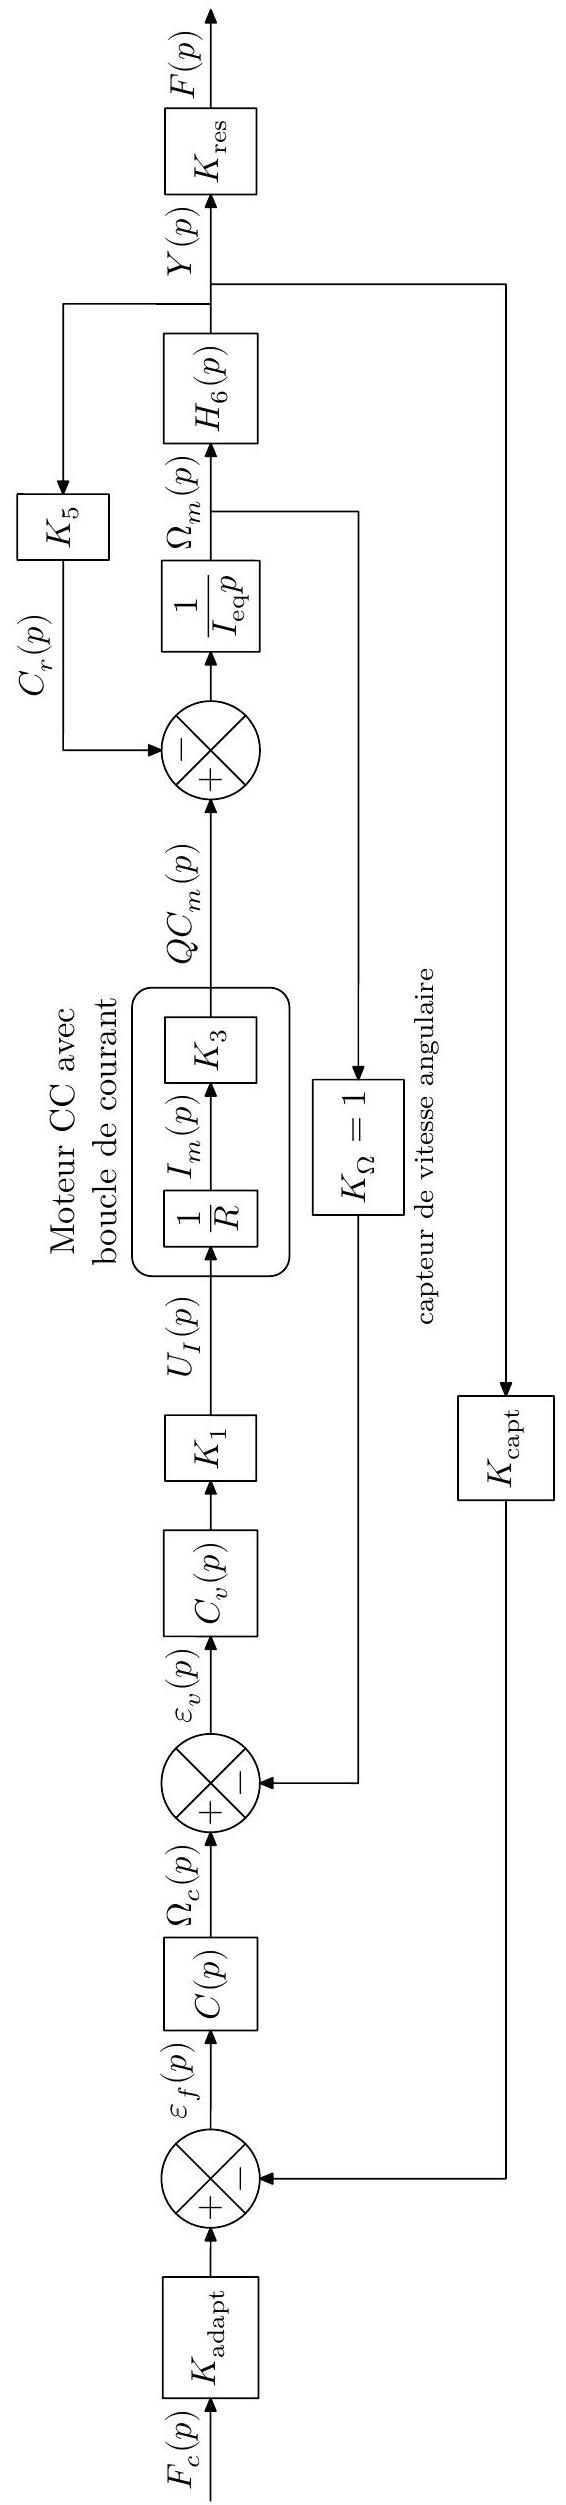
\includegraphics[width=\textwidth]{2025_09_16_5f2d7643f7e649c6833dg-09}
%\captionsetup{labelformat=empty}
%\caption{Figure 11 Schéma-blocs de l'asservissement de force développée par un actionneur linéaire placé sur le banc d'essai}
%\end{center}
%\end{figure}


\begin{figure}[!h]
\centering
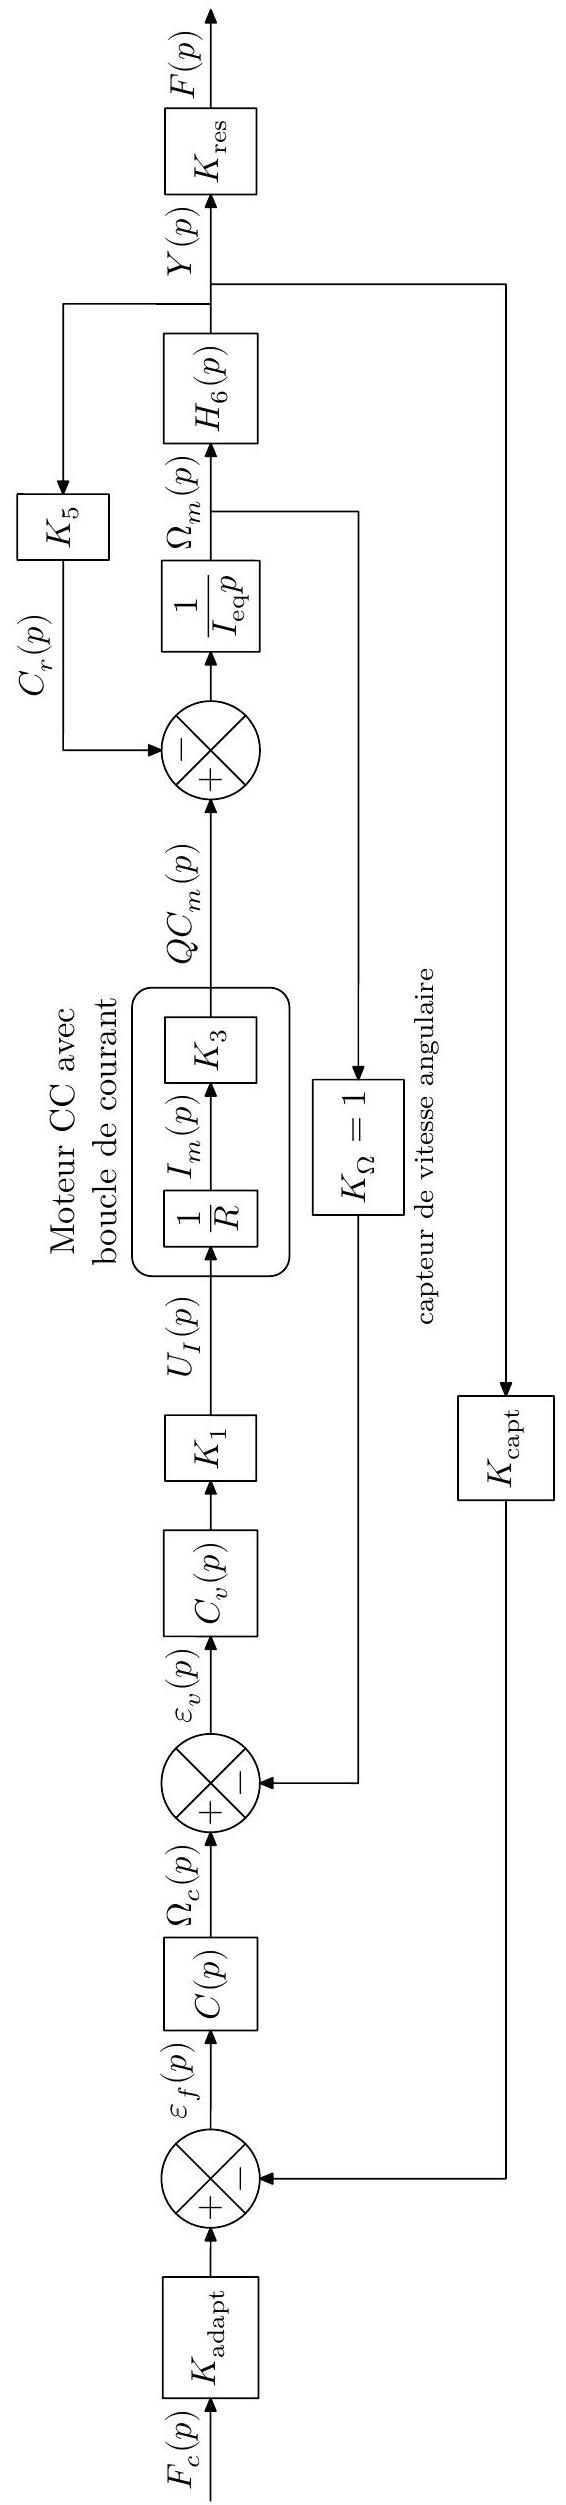
\includegraphics[width=.3\textwidth]{2025_09_16_5f2d7643f7e649c6833dg-09}
\caption{\label{ccs_mp_2023_fig_11}  Schéma-blocs de l'asservissement de force développée par un actionneur linéaire placé sur le banc d'essai}
\end{figure}

\fi


%Q 14. \\
\question{\label{ccs_mp_2023_q_14}
Après avoir transformé les équations précédentes dans le domaine de Laplace, exprimer les gains $K_{3}$ et $K_{5}$ en fonction de $Q, k_{c}$ et $T$.}
\ifprof
\begin{corrige}
Dans le domaine de Laplace et en utilisant les conditions de Heaviside, on a :
$U_I(p) = R I_m(p)$, 
$I_{\text{eq}}p \Omega_m(p) = Q \cdot C_m(p) - C_r(p)$, 
$C_r(p) = T \cdot Y(p)$, 
$C_m(p) = k_c I_m(p)$.


Ainsi on identifie dans le schéma-blocs: $\boxed{K_3 = Q \cdot k_c}$ et $\boxed{K_5 = T}$.
\end{corrige}
\else
\fi

%Q 15. \\
\question{\label{ccs_mp_2023_q_15}
Exprimer la fonction de transfert $H_{6}(p)$ en fonction de $K_{\text {trans }}$.}
\ifprof
\begin{corrige}
On a $\dot{y}(t) = K_{\text{trans}} \omega_m(t)$ soit dans le domaine de Laplace $\dfrac{K_{\text{trans}}}{p} \Omega_m(p) = Y(p)$. On identifie $\boxed{H_6(p)=\dfrac{K_{\text{trans}}}{p}}$.
\end{corrige}
\else
\fi


%Q 16. 
\question{\label{ccs_mp_2023_q_16}En supposant le système stable, déterminer l'expression de $K_{\text {adapt }}$ en fonction de $K_{\text {capt }}$ et $K_{\text {res }}$ qui assure que l'écart en régime permanent ( $\varepsilon(t \rightarrow \infty)$ ) soit nul si l'erreur en régime permanent est nulle.}
\ifprof
\begin{corrige}
On ramène la grande boucle de retour (celle avec le gain $K_{\text{capt}}$) sur la sortie $F(p)$, le gain sur la boucle de retour devient alors $\dfrac{K_{\text{capt}}}{K_{\text{res}}}$.\\

Ainsi pour valider la condition demandée il faut $\boxed{K_{\text{adapt}} = \dfrac{K_{\text{capt}}}{K_{\text{res}}}}$.


\end{corrige}
\else
\fi



%
\subsubsection{Réglage de la boucle d'asservissement de la vitesse angulaire du moteur}%III.B.2) 


\ifprof
\else

Le schéma-blocs décrivant la structure de l'asservissement de la vitesse angulaire du moteur est fourni sur la figure \ref{ccs_mp_2023_fig_12}. Cet asservissement doit respecter le cahier des charges fourni dans le tableau \ref{ccs_mp_2023_tab_04}.

%\begin{figure}[h]
%\begin{center}
%  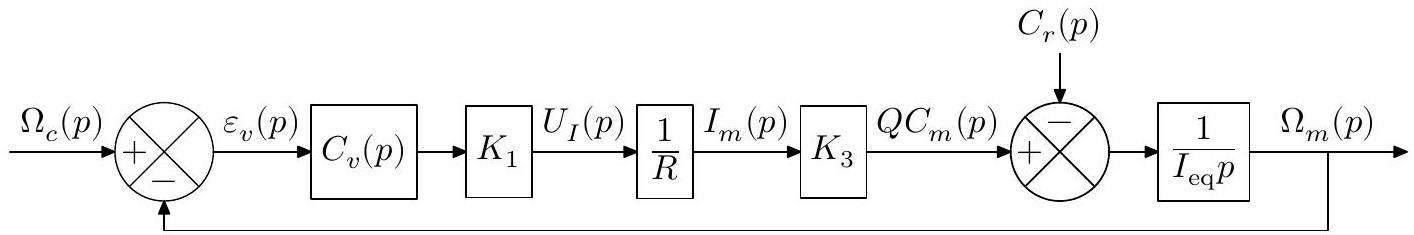
\includegraphics[width=\textwidth]{2025_09_16_5f2d7643f7e649c6833dg-10}
%\captionsetup{labelformat=empty}
%\caption{Figure 12 Schéma-blocs de la boucle d'asservissement de la vitesse angulaire du moteur électrique}
%\end{center}
%\end{figure}


\begin{figure}[!h]
\centering
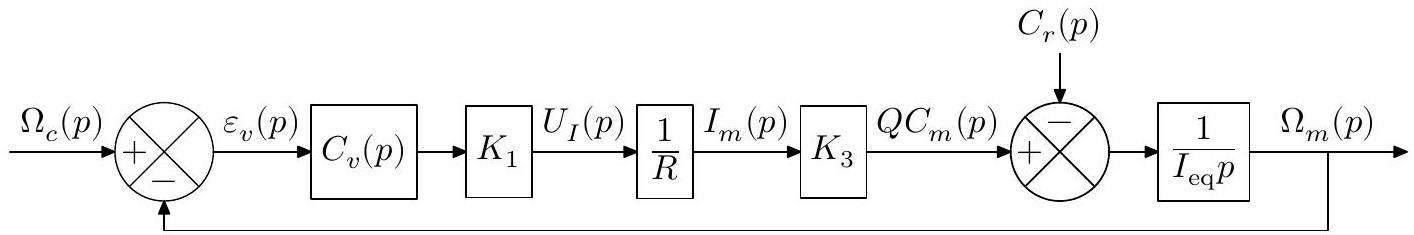
\includegraphics[width=\textwidth]{2025_09_16_5f2d7643f7e649c6833dg-10}
\caption{\label{ccs_mp_2023_fig_12}  Schéma-blocs de la boucle d'asservissement de la vitesse angulaire du moteur électrique}
\end{figure}



\begin{table}[h]
\begin{center}
\begin{tabular}{ll}
\hline
\textbf{Critère concepteur} & \textbf{Niveau} \\
\hline
Marge de phase & $\geqslant 80^{\circ}$ \\

Erreur en régime permanent pour une perturbation en échelon constante & Nulle \\

Pulsation de coupure à 0 dB & $\omega_{0 \mathrm{~dB}}=10 \mathrm{rad} \cdot \mathrm{s}^{-1}$ \\
\hline
\end{tabular}
%\captionsetup{labelformat=empty}
\caption{\label{ccs_mp_2023_tab_04}Critères concepteur pour la boucle d'asservissement de la vitesse angulaire}
\end{center}
\end{table}

Le choix d'un correcteur proportionnel intégral est fait afin de diminuer l'influence de la perturbation en couple modélisée par $C_{r}(p)$. La fonction de transfert du correcteur de la boucle d'asservissement en vitesse angulaire est noté $C_{v}(p)$, tel que

$$
C_{v}(p)=K_{i} \frac{1+\tau_{i} p}{\tau_{i} p} .
$$

On note $\indice{H}{BOv}(p)=\frac{\Omega_{m}(p)}{\varepsilon_{v}(p)}$ la fonction de transfert en boucle ouverte de l'asservissement de vitesse angulaire du moteur.
\fi

%Q 17. 
\question{\label{ccs_mp_2023_q_17}
Déterminer l'expression littérale de la phase de $\indice{H}{BOv}(\mathrm{i} \omega)$. En déduire la valeur numérique de $\tau_{i}$ respectant les critères concepteur de la boucle de vitesse.}
\ifprof
\begin{corrige}
Dans le domaine de Laplace: $H_{BOv}(p) = \dfrac{K_i K_1 K_3}{I_{\text{eq}}R} \cdot \dfrac{1 + \tau_i p}{\tau_i p^2}$.

On calcule la phase en degrés dans le domaine fréquentiel: $\varphi(\omega) = \text{Arg}\left( H_{BOv}(\text{i}\omega) \right) = \arctan(\tau_i \omega) - 180$.\\

On veut une marge de phase $M_{\varphi} = 180 + \varphi(\omega_{0\text{dB}}) \geq 80^\circ$, autrement dit $\arctan(\tau_i \omega_{0\text{dB}}) \geq 80^\circ$. Par croissance de la fonction arctan on trouve $\boxed{\tau_i \geq \dfrac{\tan(80)}{\omega_{0\text{dB}}} = 0,57\text{ s}}$
\end{corrige}
\else
\fi

\ifprof
\else

Le diagramme de Bode de la boucle ouverte $\indice{H}{B O v}(p)$, avec $K_{i}=1$ et $\tau_{i}$ déterminé à la question \ref{ccs_mp_2023_q_17}, est donné sur la figure \ref{ccs_mp_2023_fig_13}.

%\begin{figure}[h]
%\begin{center}
%  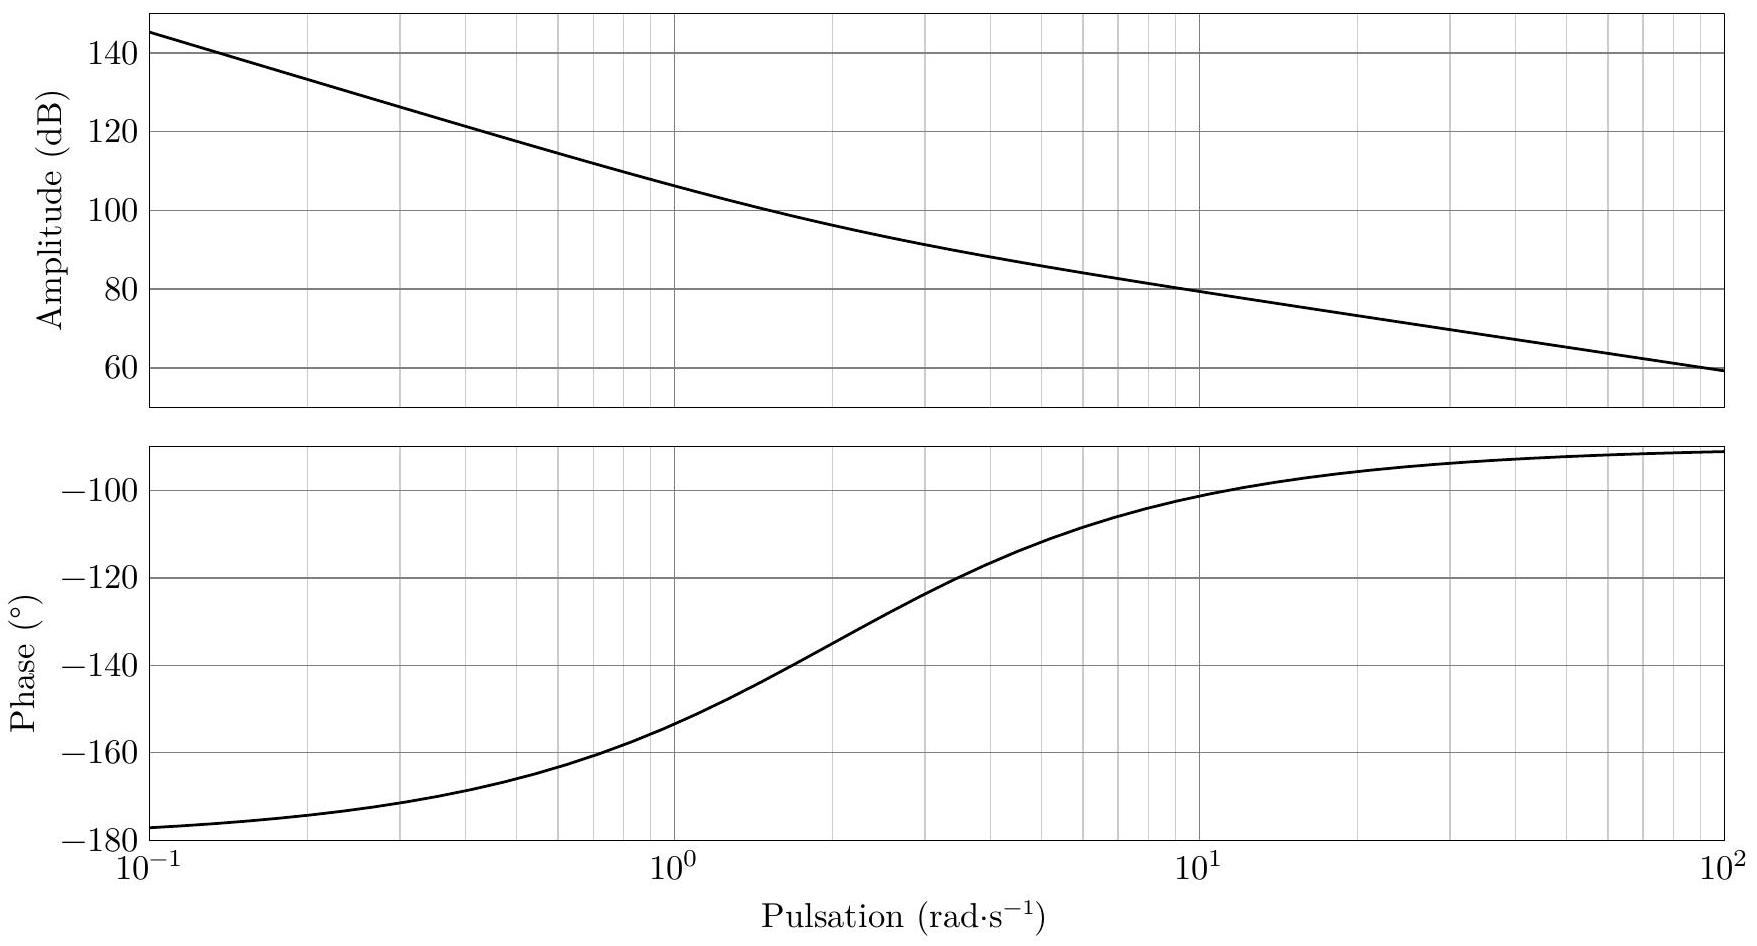
\includegraphics[width=\textwidth]{2025_09_16_5f2d7643f7e649c6833dg-10(1)}
%\captionsetup{labelformat=empty}
%\caption{Figure 13 Diagramme de Bode de \$H\_\{B O v}(p)\$\}\end{center}
%\end{figure}


\begin{figure}[!h]
\centering
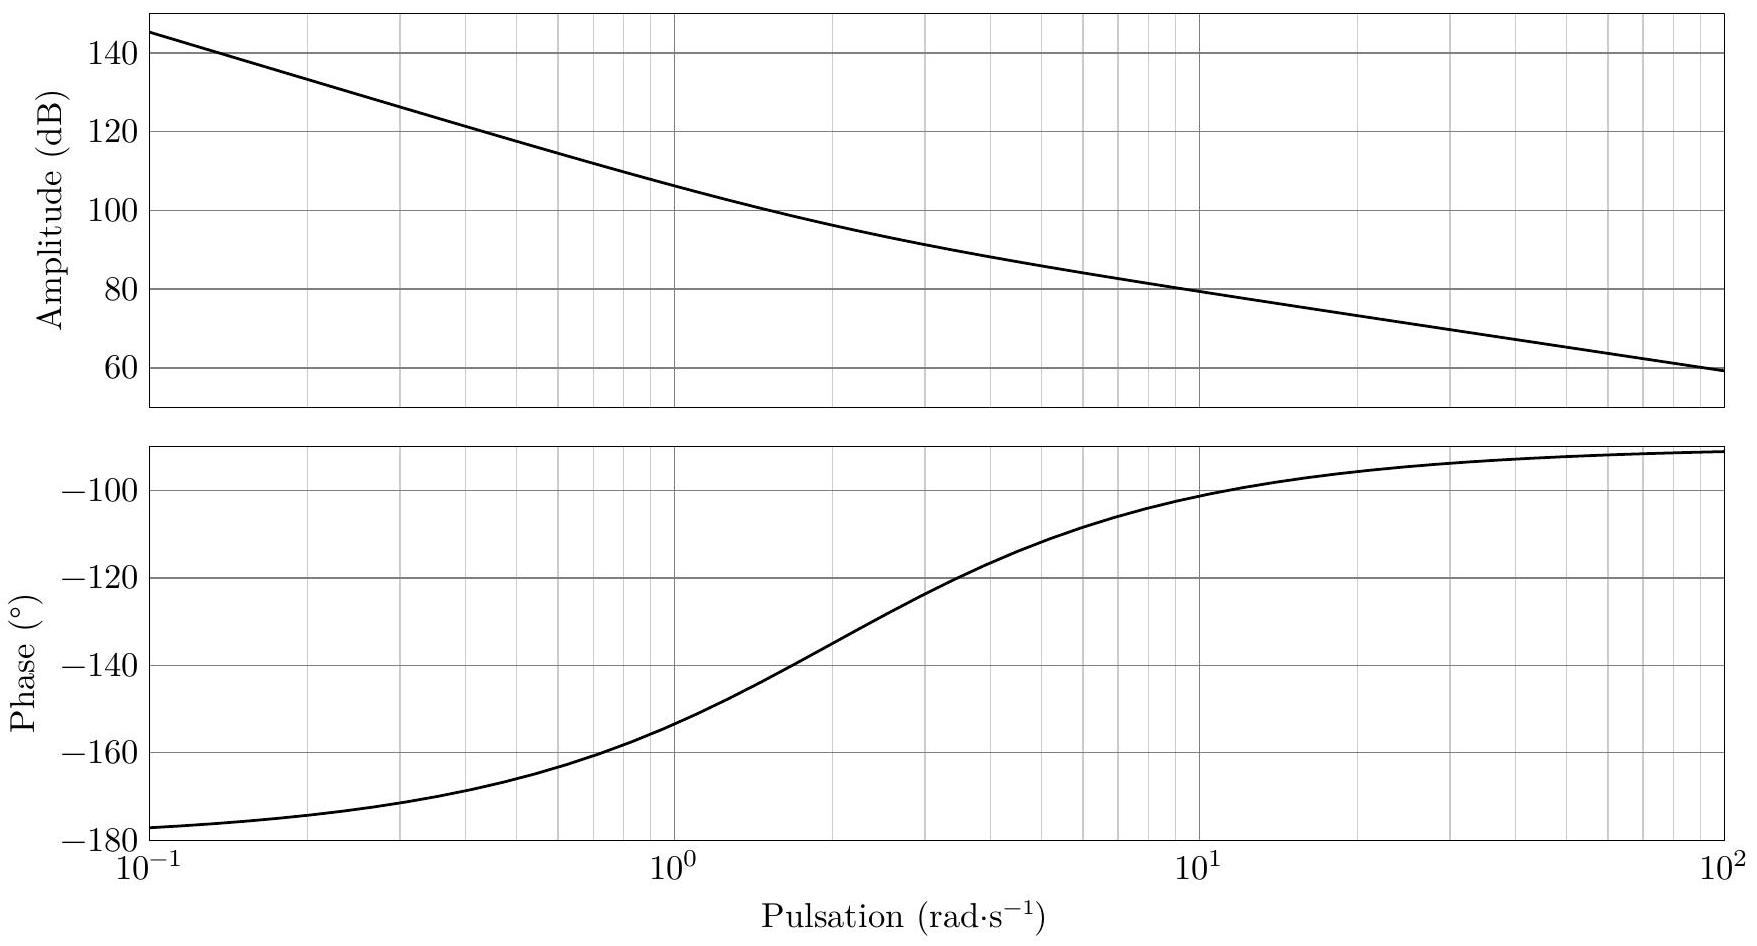
\includegraphics[width=.8\textwidth]{2025_09_16_5f2d7643f7e649c6833dg-10(1)}
\caption{\label{ccs_mp_2023_fig_13}   Diagramme de Bode de $\indice{H}{BOv}(p)$}
\end{figure}
\fi



%Q 18. 
\question{\label{ccs_mp_2023_q_18}
Déterminer la valeur numérique de $K_{i}$ afin que la boucle d'asservissement de vitesse respecte les critères concepteur du tableau \ref{ccs_mp_2023_tab_04}.}
\ifprof
\begin{corrige}
On veut une pulsation de coupure $\omega_{0\text{dB}} = 10$ rad/s, autrement dit d'après le diagramme de gain il faut diminuer le gain de 80dB environ (voir ci-dessous). Alors:

$$ 20\log(K_i) = -80 \quad \Leftrightarrow \quad \boxed{K_i = 10^{-4} \text{ V.s/rad}} $$

\begin{center}
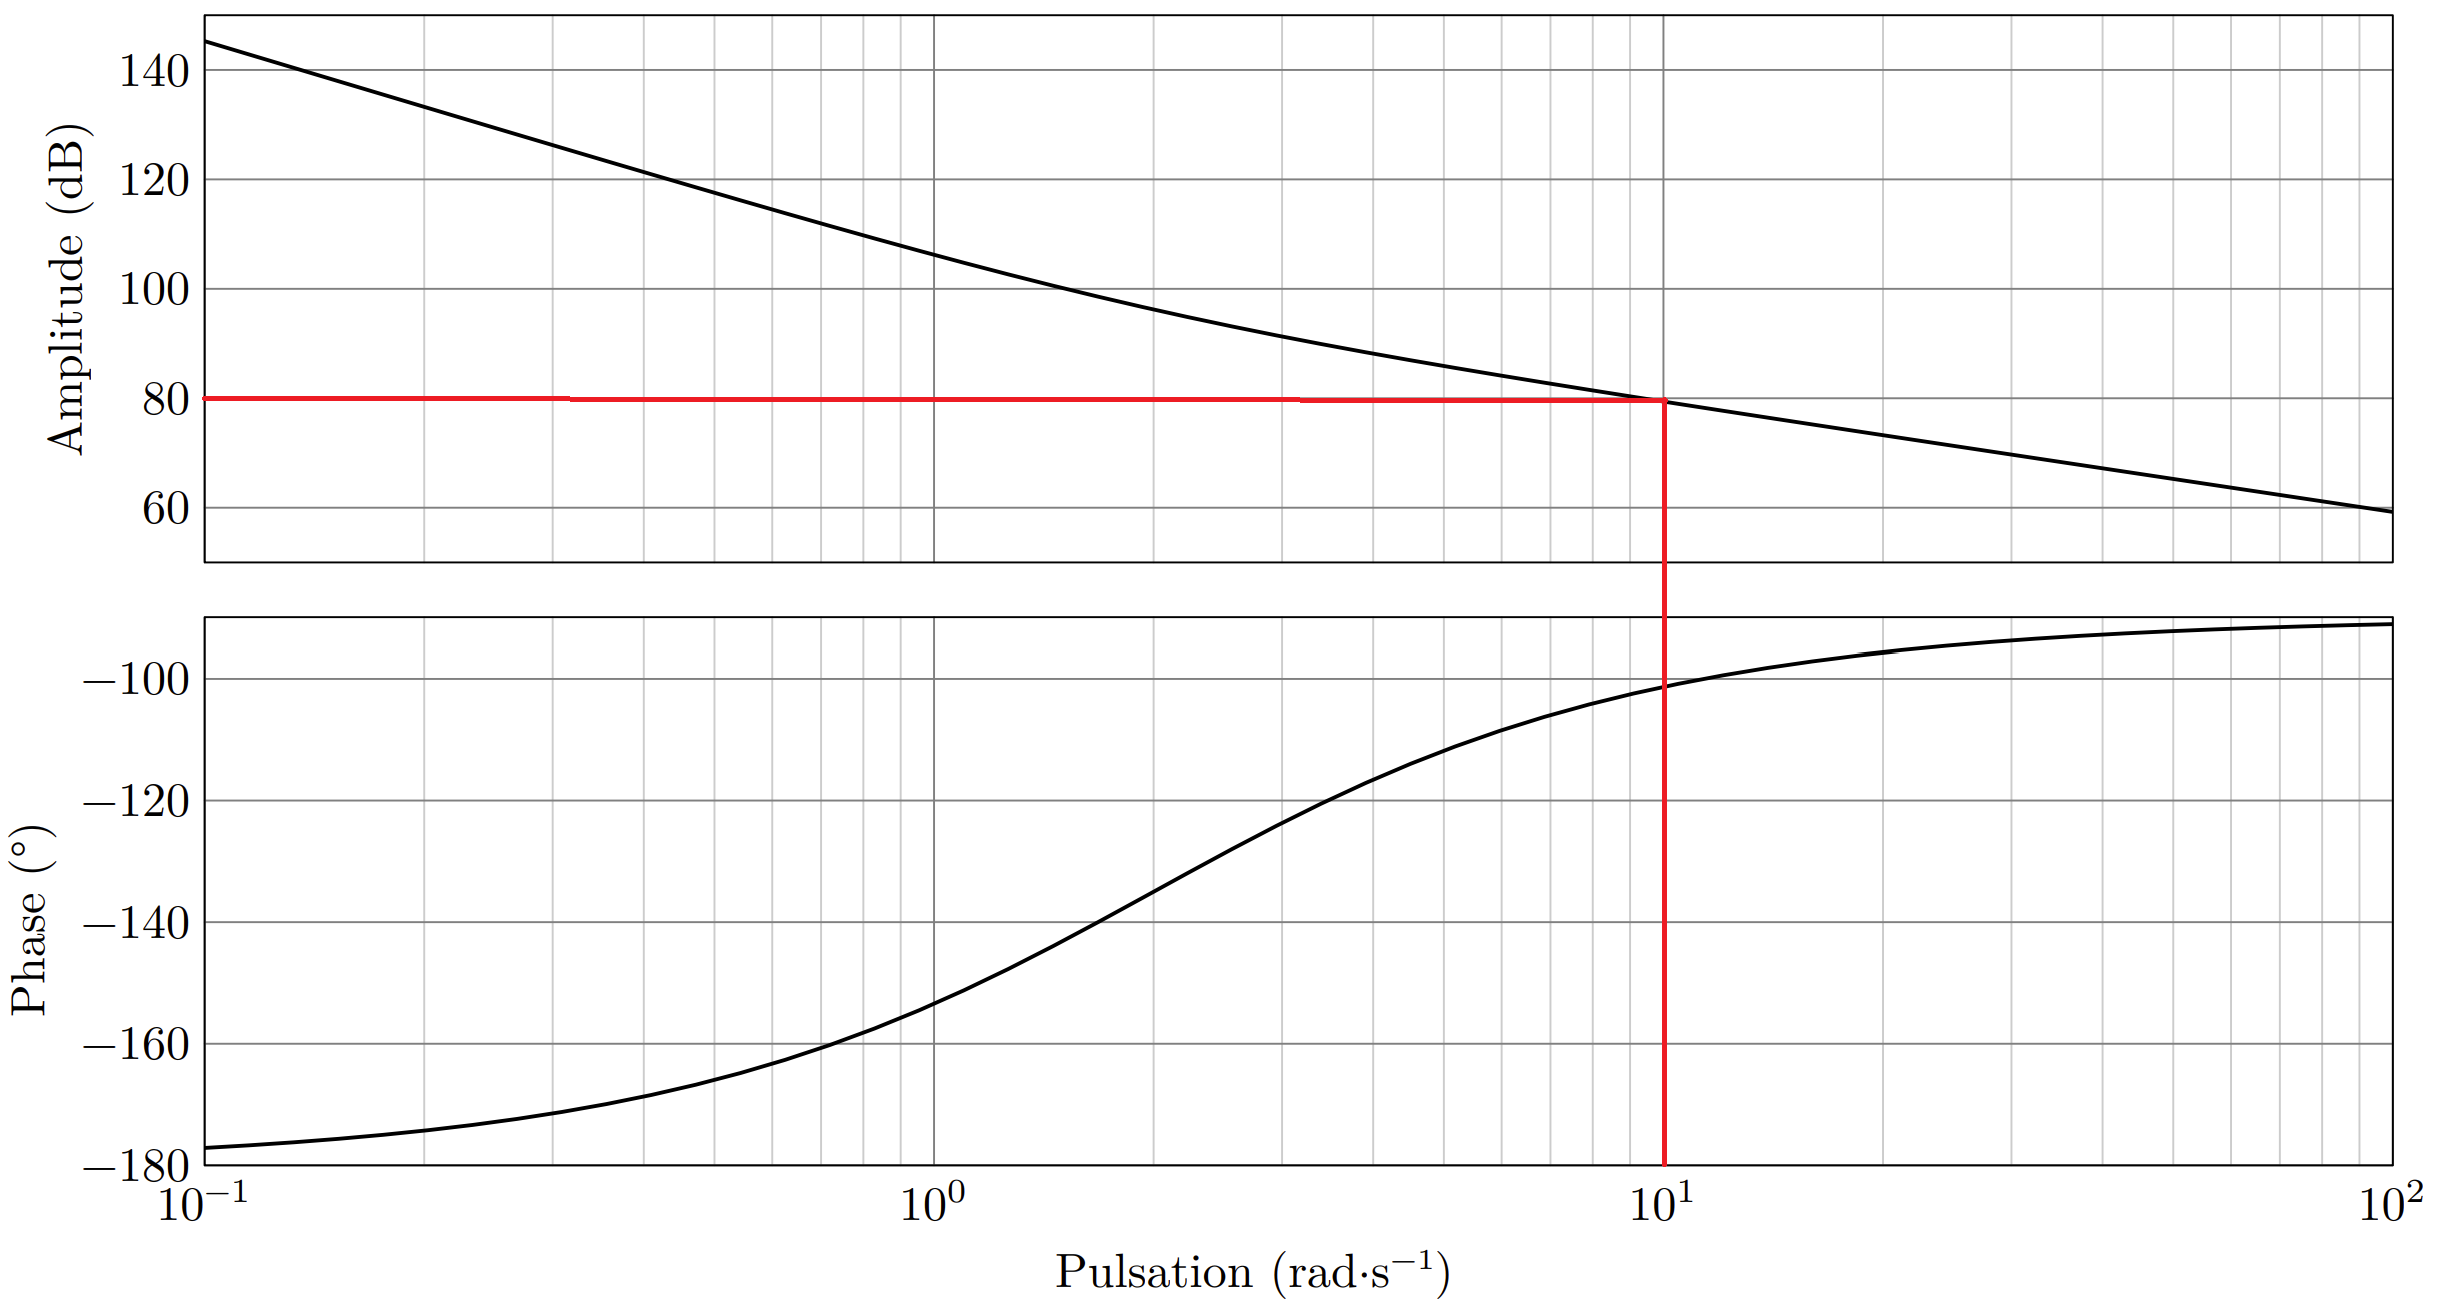
\includegraphics[width = .6\linewidth]{Bode_correcteur}
\end{center}

Tous les critères du tableau 4 sont respectés (marge de phase très légèrement inférieure à celle cherchée toutefois), le critère de précision et d'insensibilité à la perturbation l'étant forcément par la nature du correcteur PI.\\

%\textbf{Remarque:} le choix de l'unité de $K_i$ est motivé par la dimension (unitaire je pense) du gain $K_1$.


\end{corrige}
\else
\fi



\subsubsection{Simplification du modèle de connaissance}%III.B.3) 
\ifprof
\else

Il est possible de mettre le schéma-blocs de la figure \ref{ccs_mp_2023_fig_11} sous la forme du schéma-blocs de la figure \ref{ccs_mp_2023_fig_14}, afin de faciliter la prévision des performances simulées.

%\begin{figure}[h]
%\begin{center}
%  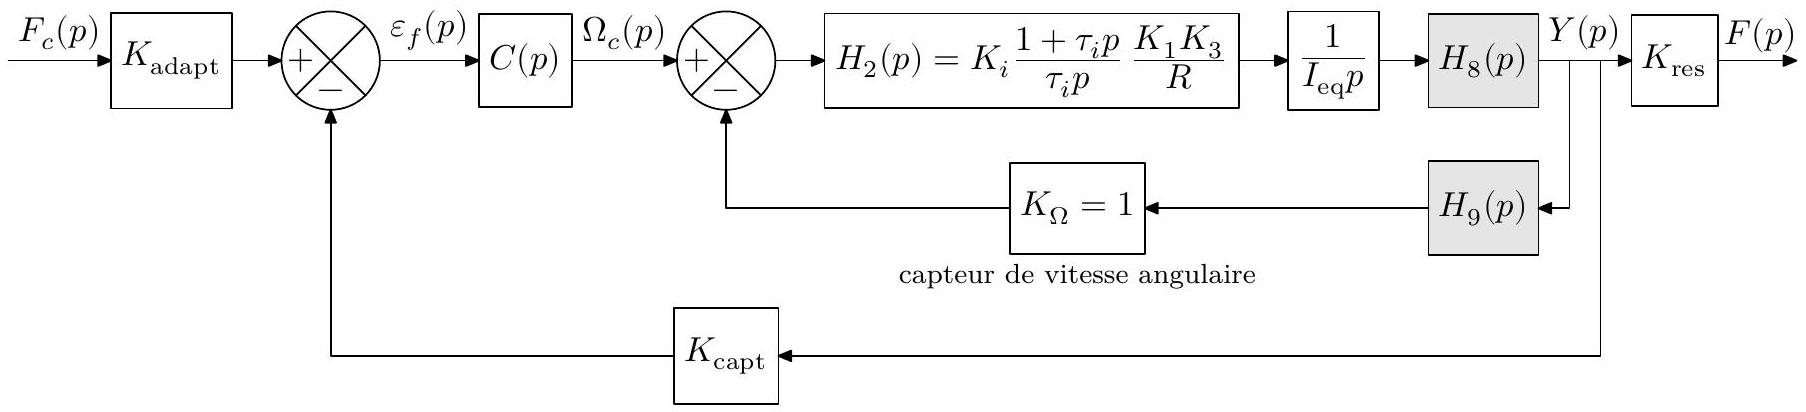
\includegraphics[width=\textwidth]{2025_09_16_5f2d7643f7e649c6833dg-11(1)}
%\captionsetup{labelformat=empty}
%\caption{Figure 14 Schéma-blocs de l'asservissement de la force développée par un actionneur linéaire}
%\end{center}
%\end{figure}


\begin{figure}[!h]
\centering
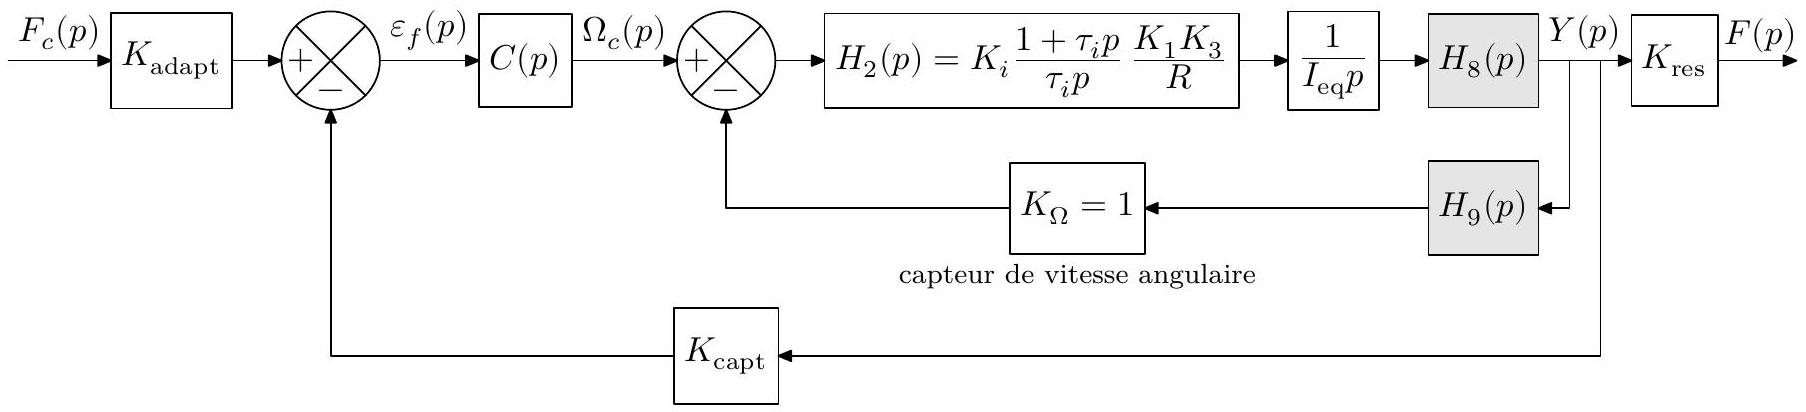
\includegraphics[width=.8\textwidth]{2025_09_16_5f2d7643f7e649c6833dg-11(1)}
\caption{\label{ccs_mp_2023_fig_14} Schéma-blocs de l'asservissement de la force développée par un actionneur linéaire }
\end{figure}
\fi



%Q 19. 
\question{\label{ccs_mp_2023_q_19}
Déterminer les fonctions de transfert $H_{8}(p)$ et $H_{9}(p)$ en fonction de $K_{5}, I_{\text {eq }}$ et $H_{6}(p)$. Ne pas remplacer $K_{5}$ et $H_{6}(p)$ par les expressions trouvées précédemment.}
\ifprof
\begin{corrige}

On décale la boucle du capteur angulaire de vitesse d'un cran vers la droite, on trouve alors immédiatement $\boxed{H_9(p) = \dfrac{1}{H_6(p)}}$.\\

On peut ensuite appliquer la formule de Black à la boucle qui possède la chaîne de retour $K_5$, on trouve $\dfrac{Y(p)}{Q C_m(p)} = \dfrac{\dfrac{H_6(p)}{I_{\text{eq}}p}}{1+ \dfrac{H_6(p)}{I_{\text{eq}}p}K_5}$, par conséquent $\boxed{H_8(p) = \dfrac{H_6(p)}{1+ \dfrac{H_6(p)}{I_{\text{eq}}p}K_5}}$.

\end{corrige}
\else
\fi

\ifprof
\else

Pour faciliter l'analyse des performances simulées, le schéma-blocs de la figure \ref{ccs_mp_2023_fig_14} est adapté afin de disposer d'un schéma-blocs à retour unitaire, tel que décrit sur la figure \ref{ccs_mp_2023_fig_15}.

%\begin{figure}[h]
%\begin{center}
%  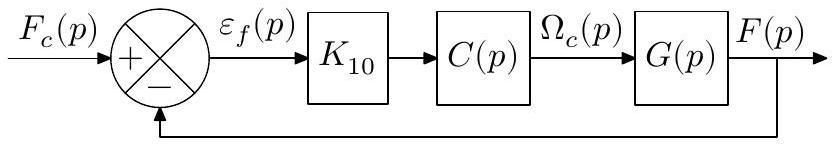
\includegraphics[width=\textwidth]{2025_09_16_5f2d7643f7e649c6833dg-11}
%\captionsetup{labelformat=empty}
%\caption{Figure 15 Schéma-blocs de l'asservissement de la force développée par un actionneur linéaire à retour unitaire}
%\end{center}
%\end{figure}


\begin{figure}[!h]
\centering
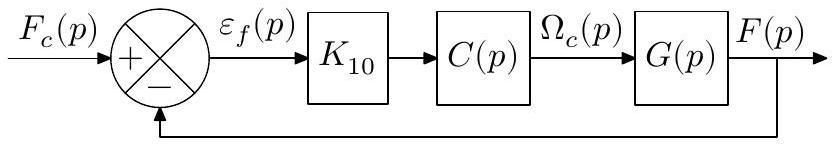
\includegraphics[width=.6\textwidth]{2025_09_16_5f2d7643f7e649c6833dg-11}
\caption{\label{ccs_mp_2023_fig_15} Schéma-blocs de l'asservissement de la force développée par un actionneur linéaire à retour unitaire}
\end{figure}
\fi

%Q 20. \\
\question{\label{ccs_mp_2023_q_20}
Déterminer l'expression du gain $K_{10}$ en fonction de $K_{\text {capt }}$ et de $K_{\text {res }}$.}
\ifprof
\begin{corrige}
On a déjà montré en question \ref{ccs_mp_2023_q_16} que $K_{\text{adapt}} = \dfrac{K_{\text{capt}}}{K_{\text{res}}}$, en factorisant dans la figure \ref{ccs_mp_2023_fig_14} on trouve le $\boxed{K_{10} = \dfrac{K_{\text{capt}}}{K_{\text{res}}}}$ de la figure \ref{ccs_mp_2023_q_15}.\\

\textbf{Remarque:} l'écart $\varepsilon_f(p)$ de la figure \ref{ccs_mp_2023_fig_15} ne peut pas être le même que celui de la figure 14. En effet dans la figure \ref{ccs_mp_2023_fig_14} on a $\varepsilon_f(p) = \dfrac{K_{\text{capt}}}{K_{\text{res}}}\left( F_c(p) - F(p) \right)$ et dans la figure 15 $\varepsilon_f(p) = F_c(p) - F(p)$. Le $\varepsilon_f(p)$ de la figure \ref{ccs_mp_2023_fig_15} aurait dû se trouver derrière le gain $K_{10}$.


\end{corrige}
\else
\fi


%Q 21. 

\question{\label{ccs_mp_2023_q_21}
Déterminer la fonction de transfert $G(p)$ en fonction de $H_{2}(p), I_{\text {eq }}, H_{8}(p), H_{9}(p)$ et $K_{\text {res }}$. Ne pas remplacer $H_{2}(p), H_{8}(p)$ et $H_{9}(p)$ par les expressions trouvées précédemment.\\}
\ifprof
\begin{corrige}
Par formule de Black sur la boucle interne on trouve $\boxed{G(p) = \dfrac{H_2(p) H_8(p)}{I_{\text{eq}}p + H_2(p)H_8(p)H_9(p)}}$.
\end{corrige}
\else
\fi

\ifprof
\else

Pour la suite, on donne la fonction de transfert $G(p)$, obtenue avec les valeurs de réglage correctes déterminées aux questions \ref{ccs_mp_2023_q_17} et \ref{ccs_mp_2023_q_18},
$$
G(p)=\frac{F(p)}{\Omega_{c}(p)}=\frac{1+\tau_{i} p}{p} \frac{1,2 \times 10^{-5}}{2 \times 10^{-4}+9,7 \times 10^{-5} p+5,3 \times 10^{-6} p^{2}} .
$$
\fi

\subsubsection{Analyse des performances de l'asservissement en force développée par un actionneur linéaire}%III.B.4) 

\ifprof
\else

Il est proposé dans cette section d'analyser les performances simulées de l'asservissement en force dont un extrait du cahier des charges est présenté dans le tableau \ref{ccs_mp_2023_tab_05}.

\begin{table}[h]
\begin{center}
\begin{tabular}{llll}
\hline
\textbf{Id} & \textbf{Exigence} & \textbf{Critère} & \textbf{Niveau} \\
\hline
\multirow[t]{3}{*}{Id1.1} & \multirow[t]{3}{*}{Stabilité} & Marge de phase & $\geqslant 60^{\circ}$ \\

 &  & Marge de gain & $>20 \mathrm{~dB}$ \\

 &  & Dépassement maximal & < 2,5\% \\
\hline
Id1.2 & Précision & Erreur en régime permanent pour une entrée en échelon & < 1\% \\
\hline
\multirow[t]{2}{*}{Id1.3} & \multirow[t]{2}{*}{Rapidité} & Temps de réponse à $5 \%$ pour une consigne en échelon de force de 40 N & $\operatorname{tr}_{5 \%}<1 \mathrm{~s}$ \\

 &  & Vitesse maximale de montée de la force de traction & $100 \mathrm{~N} \cdot \mathrm{~s}^{-1}$ \\
\hline
\end{tabular}
%\captionsetup{labelformat=empty}
\caption{\label{ccs_mp_2023_tab_05}Extrait du cahier des charges fonctionnel de l'actionneur linéaire sur le banc d'essai}
\end{center}
\end{table}

On note $\indice{H}{B O f}(p)=\frac{F(p)}{\varepsilon_{f}(p)}$ la fonction de transfert en boucle ouverte de l'asservissement en force développé par un actionneur linéaire. Dans un premier temps, le choix d'un correcteur proportionnel $C(p)=K_{\text {cor }}$ est réalisé. Le diagramme de Bode de la fonction de transfert $\indice{H}{B O f}(p)=\frac{F(p)}{\varepsilon_{f}(p)}=K_{\text {cor }} K_{10} G(p)$, avec $K_{\text {cor }}=1$ et la valeur de $\tau_{i}$ déterminée à la question \ref{ccs_mp_2023_q_17}, est donné sur la figure \ref{ccs_mp_2023_fig_16} .

%\begin{figure}[h]
%\begin{center}
%  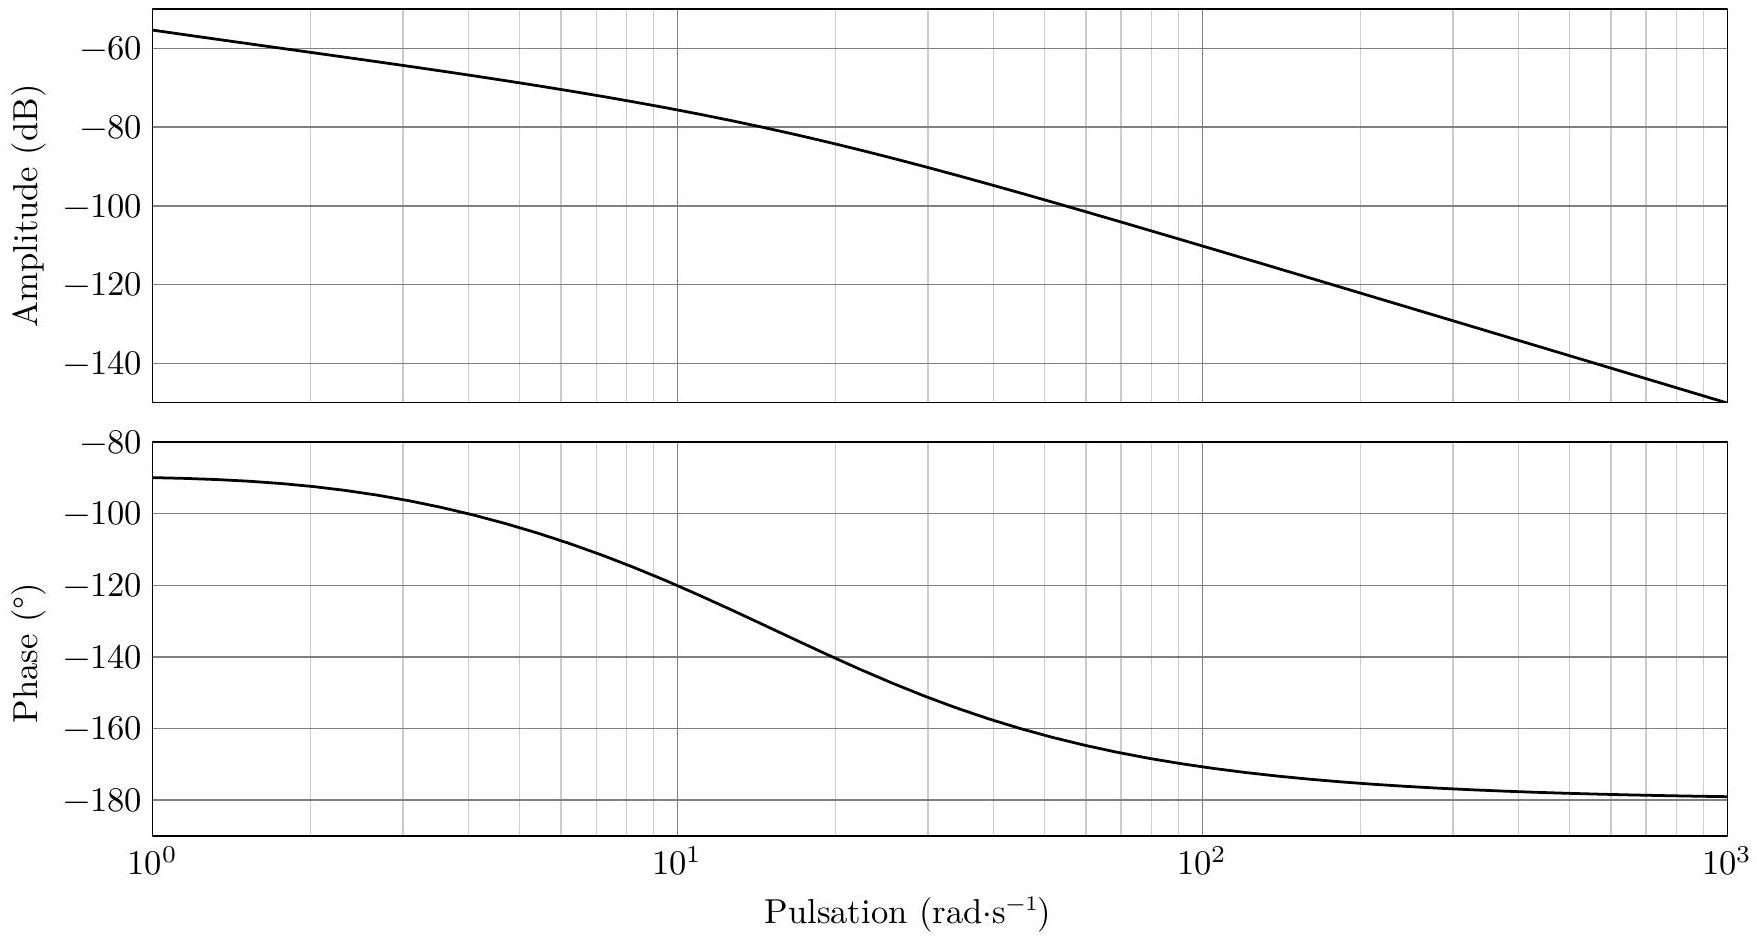
\includegraphics[width=\textwidth]{2025_09_16_5f2d7643f7e649c6833dg-12(1)}
%\captionsetup{labelformat=empty}
%\caption{Figure 16 Diagramme de Bode de \$H\_\{B O f}(p)\$\}
%\end{center}
%\end{figure}


\begin{figure}[!h]
\centering
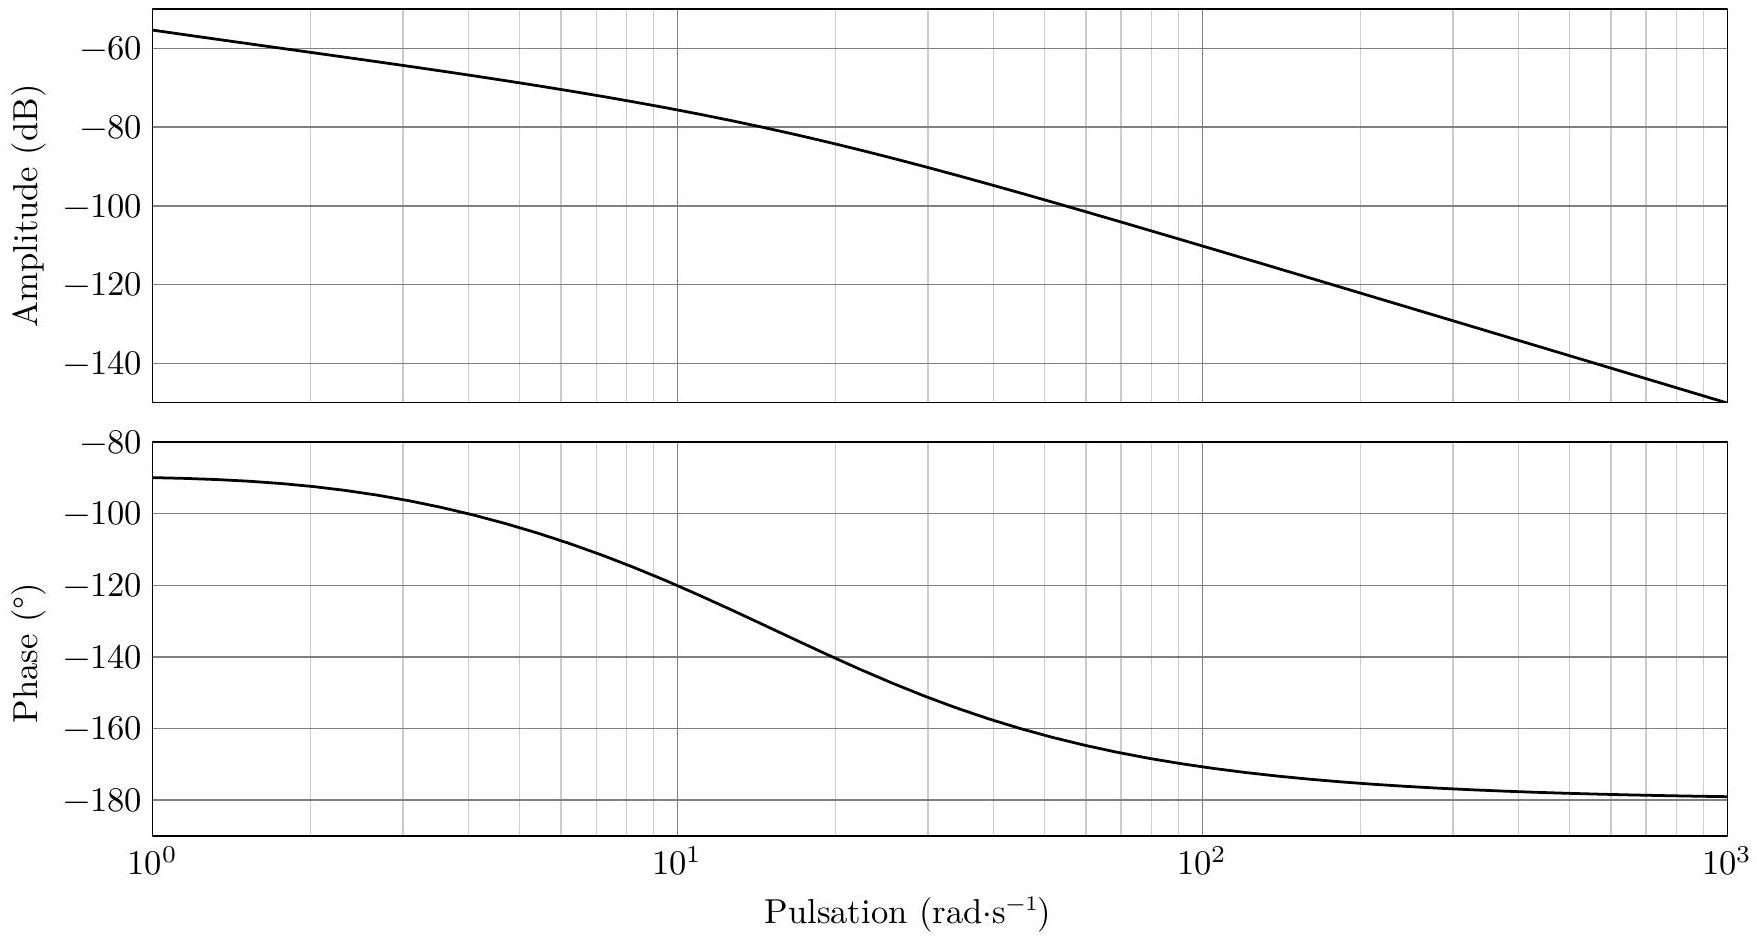
\includegraphics[width=\textwidth]{2025_09_16_5f2d7643f7e649c6833dg-12(1)}
\caption{\label{ccs_mp_2023_fig_16}  Diagramme de Bode de $\indice{H}{BO f}(p)$}
\end{figure}

\fi

%Q 22. \\
Les courbes sur la figure \ref{ccs_mp_2023_fig_17} représentent les réponses temporelles du modèle de connaissance de la figure \ref{ccs_mp_2023_fig_11}, avec les correcteurs $C_{v}(p)$ et $C(p)$ correctement réglés, et de l'expérimentation sur le banc d'essai pour une consigne en échelon de force de \SI{40}{N}.

\question{\label{ccs_mp_2023_q_22}
Déterminer la valeur numérique limite de $K_{\text {cor }}$ afin que la boucle d'asservissement de force respecte les critères de marge de phase et de gain du tableau \ref{ccs_mp_2023_tab_05}.}
\ifprof
\begin{corrige}
La marge de gain est infinie ici car la phase n'atteint jamais $-180^\circ$, regardons la marge de phase. Elle doit être de $60^\circ$ minimum, autrement dit il faut que la pulsation de coupure se situe à la phase $-120^\circ$ au maximum. Il faut alors augmenter le gain de 75dB minimum pour satisfaire le critère de marge de phase. Donc:

$$ 20\log(K_{\text{corr}}) \geq + 75 \quad \Leftrightarrow \quad  \boxed{K_{\text{corr}} \geq 10^{\frac{75}{20}} \approx 5624 \text{rad/(s.V)}}$$
\end{corrige}
\else
\fi


%\begin{figure}[h]
%\begin{center}
%  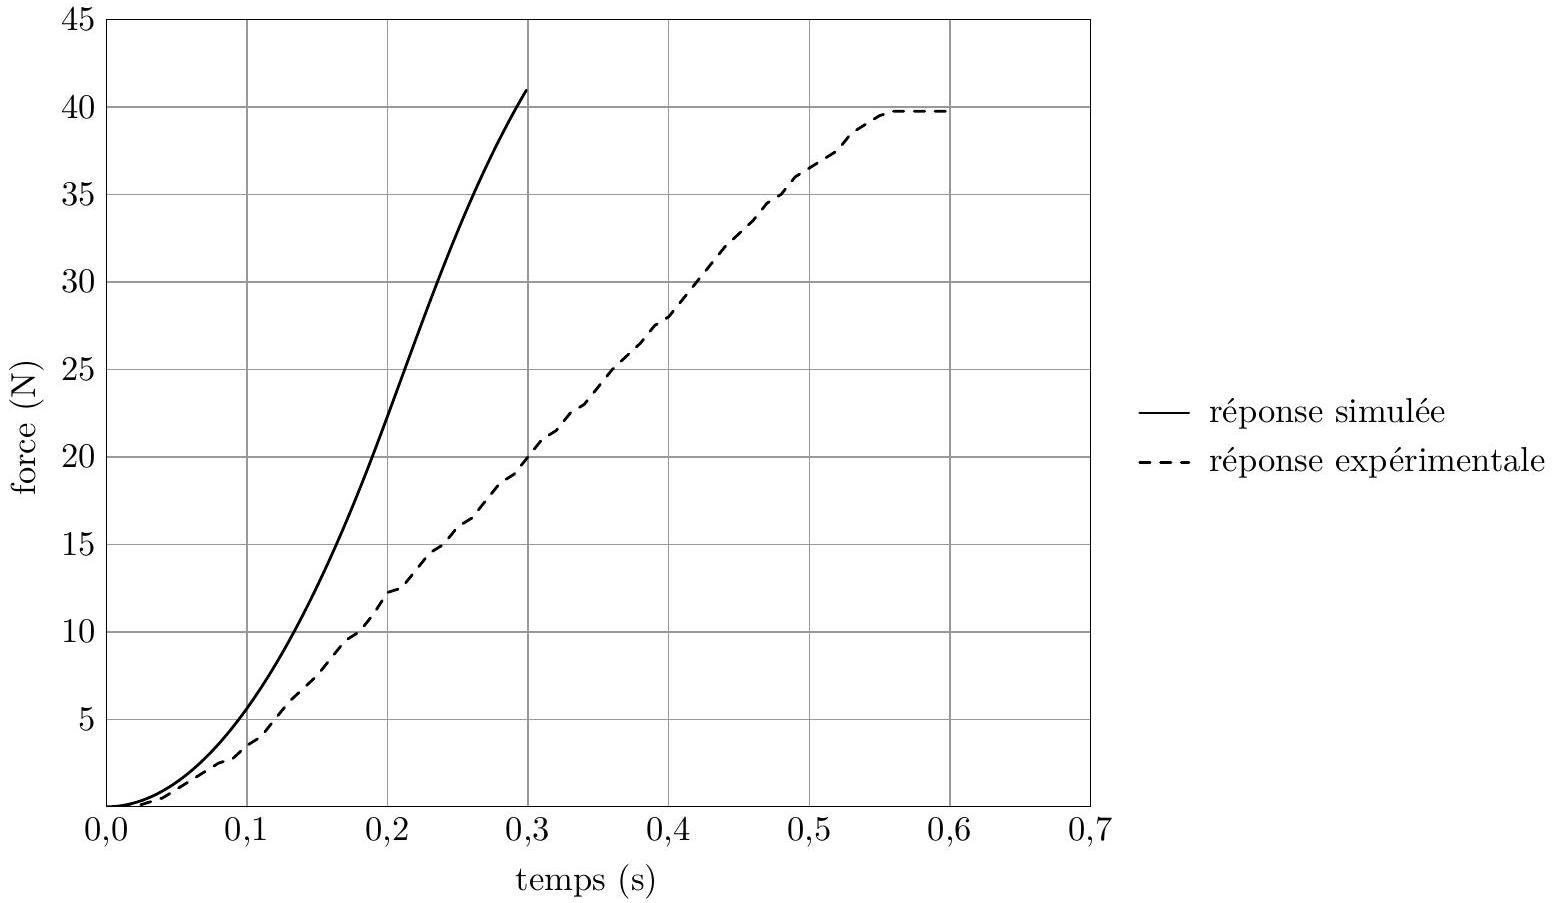
\includegraphics[width=\textwidth]{2025_09_16_5f2d7643f7e649c6833dg-12}
%\captionsetup{labelformat=empty}
%\caption{Figure 17 Réponses temporelles du modèle et expérimentale, pour une consigne en échelon de force de 40 N}
%\end{center}
%\end{figure}


\ifprof
\else


\begin{figure}[!h]
\centering
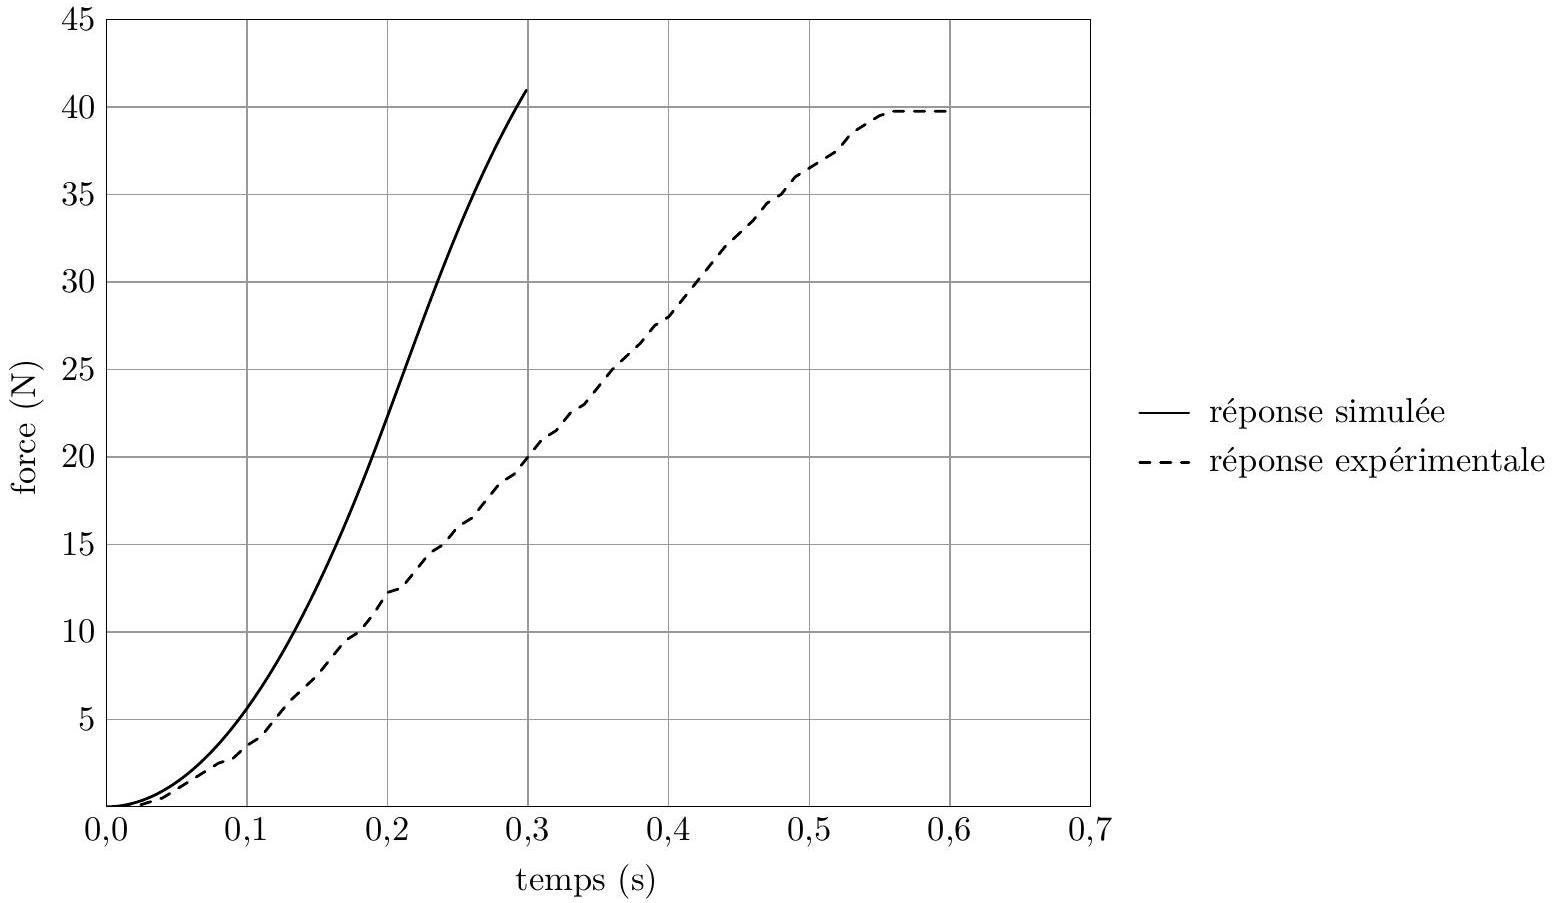
\includegraphics[width=\textwidth]{2025_09_16_5f2d7643f7e649c6833dg-12}
\caption{\label{ccs_mp_2023_fig_17} Réponses temporelles du modèle et expérimentale, pour une consigne en échelon de force de \SI{40}{N}}
\end{figure}

\fi



%Q 23. 
\question{\label{ccs_mp_2023_q_23}
Quel critère du tableau des exigences (tableau \ref{ccs_mp_2023_tab_05}) n'est pas pris en compte dans le modèle de connaissance? D'après la courbe expérimentale, ce critère est-il respecté par le système réel ?}
\ifprof
\begin{corrige}
Sur la figure \ref{ccs_mp_2023_fig_17} la simulation s'arrête quand le dépassement vaut 2,5\%, soit 41N. On ne peut pas évaluer le temps de réponse du système puisque le régime stationnaire pour une consigne en échelon n'est pas atteint.\\

Sur le relevé expérimental ce temps de réponse est clairement inférieur à la valeur 1s demandée par le cahier des charges et il n'y a pas de dépassement (saturation à 40N). Le cahier des charges concernant le temps de réponse à 5\% est validé expérimentalement.\\

La vitesse de montée expérimentale vaut environ $\dfrac{36 - 4}{0,5 -0,1} = 80\text{N/s} < 100\text{N/s}$ donc le critère de vitesse de montée est aussi respecté. Toutefois la vitesse de montée maximale relevée sur la courbe de simulation vaut environ $\dfrac{41 - 7}{0,28 -0,12} = 212\text{N/s} > 100\text{N/s}$, le critère de vitesse en montée n'est pas respecté lors de la simulation.  

\begin{center}
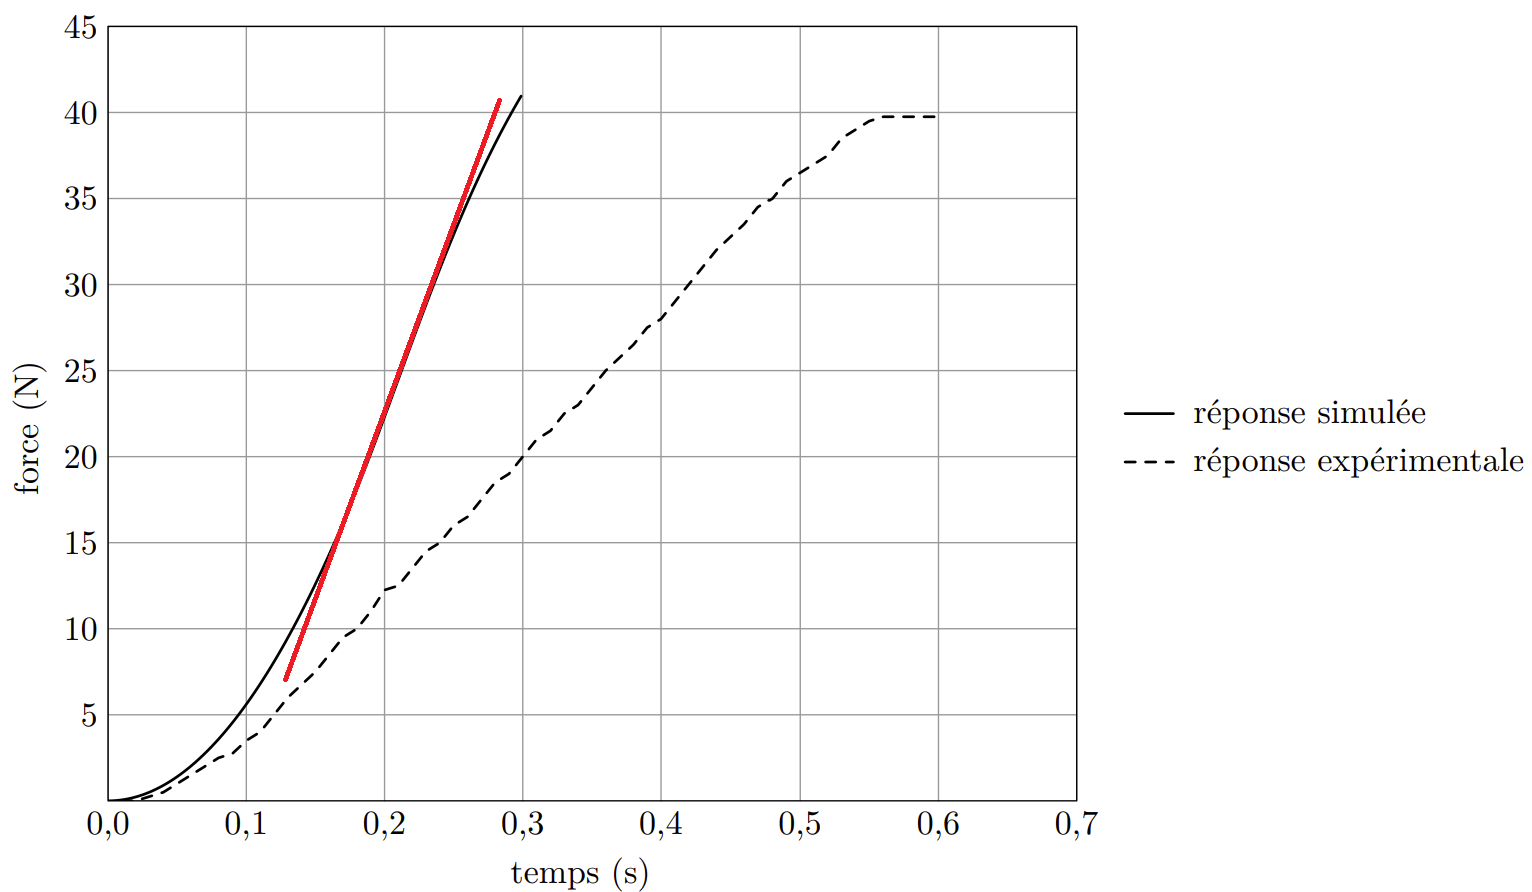
\includegraphics[width = .6\linewidth]{Vitesse_montee}
\end{center}

\end{corrige}
\else
\fi

%
%
%\subsubsection{ Amélioration du modèle. Mise en place d'une limitation en vitesse angulaire}%III.B.5)
%Pour améliorer le modèle de connaissance et le valider, la comparaison entre la réponse simulée issue du modèle de connaissance amélioré et la réponse expérimentale sera traitée par résolution numérique informatique. Le langage de programmation utilisé est Python.
%
%%\begin{figure}[h]
%%\begin{center}
%%  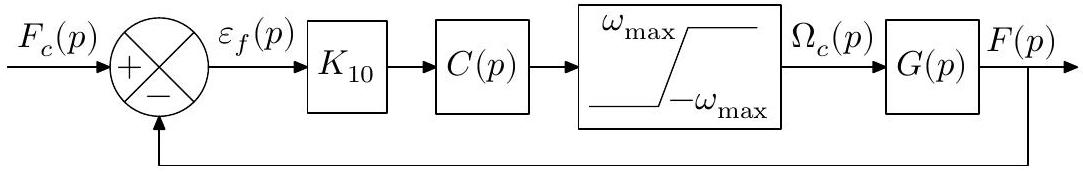
\includegraphics[width=\textwidth]{2025_09_16_5f2d7643f7e649c6833dg-13}
%%\captionsetup{labelformat=empty}
%%\caption{Figure 18 Schéma-blocs de l'asservissement de force développée par l'actionneur linéaire avec limitation de la vitesse angulaire}
%%\end{center}
%%\end{figure}
%
%
%\begin{figure}[!h]
%\centering
%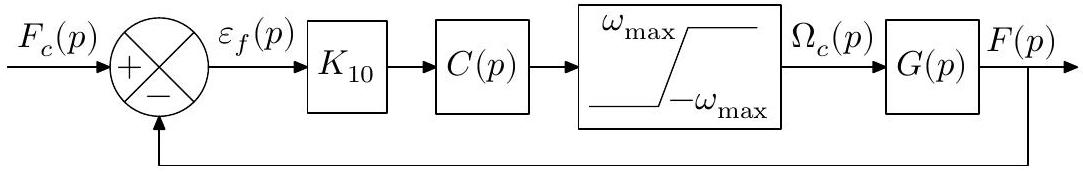
\includegraphics[width=.7\textwidth]{2025_09_16_5f2d7643f7e649c6833dg-13}
%\caption{\label{ccs_mp_2023_fig_18}  Schéma-blocs de l'asservissement de force développée par l'actionneur linéaire avec limitation de la vitesse angulaire}
%\end{figure}
%
%
%
%\textbf{Notations et hypothèses:}
%
%\begin{itemize}
%  \item $f(t)$ est la grandeur de sortie de l'asservissement en force, de variable de Laplace $F(p)$;
%  \item $f_{c}(t)$ est la grandeur de consigne de l'asservissement en force, de variable de Laplace $F_{c}(p)$;
%  \item $\omega_{c}(t)$ est la commande de vitesse angulaire du moteur, de variable de Laplace $\Omega_{c}(p)$;
%  \item la dérivée première temporelle d'une fonction $h(t)$ est notée $\dot{h}(t)$ et sa dérivée seconde $\ddot{h}(t)$;
%  \item les conditions de Heaviside sont supposées vérifiées, soient $f(t=0)=0$ et $\dot{f}(t=0)=0$.\\
%a) Cadre général de la résolution numérique d'un problème de Cauchy
%\end{itemize}
%
%Pour déterminer numériquement la solution $E(t)$ d'une équation différentielle, il faut préalablement la mettre sous la forme d'un problème de Cauchy :
%
%$$
%\dot{E}(t)=F_{\text {Cauchy }}(E(t), t) \quad \text { avec } \quad E(t=0)=E_{0} .
%$$
%
%$E(t)$ est appelé vecteur d'états à l'instant $t, \dot{E}(t)$ représente le vecteur composé des dérivées premières des états par rapport au temps $t, F_{\text {Cauchy }}$ la fonction de Cauchy et $E_{0}$ le vecteur d'états des conditions initiales.\\
%Le problème étant décrit sous la forme de Cauchy, la résolution numérique peut être menée par un schéma numérique du type Euler explicite ou en utilisant la fonction odeint de la bibliothèque scipy.\\
%b) Problème de Cauchy lié à l'équation différentielle associée à $G(p)$
%
%Compte-tenu du correcteur $C_{v}(p)$ de la boucle d'asservissement de la vitesse angulaire du moteur électrique réglé aux questions \ref{ccs_mp_2023_q_17} et \ref{ccs_mp_2023_q_18}, il est possible de simplifier la fonction de transfert $G(p)$. L'équation différentielle associée à $G(p)$ simplifiée s'écrit
%
%$$
%\ddot{f}(t)+18 \dot{f}(t)=1,18 \omega_{c}(t) .
%$$
%
%Dans le cadre de la résolution de l'équation différentielle globale liée à l'asservissement de force développée par un actionneur linéaire (figure \ref{ccs_mp_2023_fig_18}), la vitesse angulaire de consigne $\omega_{c}(t)$ est une fonction du temps inconnue à ce stade.\\
%Le vecteur d'états associé à l'étude de $G(p)$ retenu est $E(t)=\binom{f(t)}{\dot{f}(t)}$, ainsi $\dot{E}(t)=\binom{\dot{f}(t)}{\ddot{f}(t)}=G\left(E(t), \omega_{c}(t), t\right)$.\\
%%Q 24. \\
%\question{\label{ccs_mp_2023_q_24}
%Déterminer la fonction $G\left(E(t), \omega_{c}(t), t\right)$, associée à $G(p)$.}
%\ifprof
%\begin{corrige}
%\end{corrige}
%\else
%\fi
%
%
%%Q 25. 
%\question{\label{ccs_mp_2023_q_25}
%Écrire en langage Python la fonction $\mathrm{G}(\mathrm{E}, \mathrm{wc}, \mathrm{t})$ qui implémente la fonction $G\left(E(t), \omega_{c}(t), t\right)$. Cette fonction renvoie une liste de deux nombres à virgule flottante et prend en paramètres}
%\begin{itemize}
%  \item E, une liste de deux nombres représentant le vecteur d'états ;
%  \item wc, un nombre représentant la consigne de vitesse angulaire du moteur ;
%  \item t, un nombre représentant le temps.\\
%c) Problème de Cauchy lié au schéma-blocs de la figure \ref{ccs_mp_2023_fig_18} sans la limitation en vitesse angulaire
%\end{itemize}
%\ifprof
%\begin{corrige}
%\end{corrige}
%\else
%\fi
%
%
%
%Le correcteur de la boucle d'asservissement de la force développée par un actionneur linéaire est un correcteur proportionnel tel que $C(p)=K_{\text {cor }}$. Ainsi, en l'absence de limitation, la grandeur $\omega_{c}(t)$ est telle que
%
%$$
%\omega_{c}(t)=K_{\operatorname{cor}} K_{10} \varepsilon_{f}(t)=K_{\operatorname{cor}} K_{10}\left(f_{c}(t)-f(t)\right) .
%$$
%
%Il reste à exprimer la fonction de Cauchy pour la boucle fermée de l'asservissement de force
%
%$$
%\dot{E}(t)=\binom{\dot{f}(t)}{\ddot{f}(t)}=F B F s l(E(t), t) .
%$$
%
%On considère dès à présent que la consigne de force $f_{c}(t)$ est un échelon d'amplitude $F_{\text {cons }}$, prise égale à 40 N .\\
%
%\question{\label{ccs_mp_2023_q_26}
%Recopier et compléter le programme Python de la figure \ref{ccs_mp_2023_fig_19} implémentant la fonction FBFsl qui renvoie une liste de deux nombres et prend en paramètres :}
%\begin{itemize}
%  \item E, une liste de deux nombres représentant le vecteur d'états ;
%  \item t, un nombre représentant le temps.
%\end{itemize}
%
%\ifprof
%\begin{corrige}
%\end{corrige}
%\else
%\fi
%
%
%
%
%
%
%\begin{figure}[!h]
%\begin{lstlisting}
%def FBFsl(E, t):
%    Fcons = 40 # échelon de consigne de 40 N
%    K10 = 0.0277 # adaptation
%    Kcor = 5400 # gain du correcteur proportionnel
%    wc = à compléter
%    # Compléter en terminant la fonction.
%\end{lstlisting}
%\caption{\label{ccs_mp_2023_fig_19}  Programme de calcul de la fonction \lstinline{FBFsl}, à compléter}
%\end{figure}
%
%
%d) Problème de Cauchy lié au schéma-blocs de la figure \ref{ccs_mp_2023_fig_18} avec la limitation en vitesse angulaire
%
%La consigne de vitesse angulaire du moteur électrique doit être limitée, conformément au schéma-blocs de la figure \ref{ccs_mp_2023_fig_18}.\\
%
%
%%Q 27. 
%\question{\label{ccs_mp_2023_q_27}
%Recopier et compléter le programme Python de la figure \ref{ccs_mp_2023_fig_20} implémentant la fonction FBFal qui renvoie une liste de deux nombres et prend en compte la limitation de la consigne de vitesse angulaire du moteur.}
%\ifprof
%\begin{corrige}
%\end{corrige}
%\else
%\fi
%
%
%
%
%\begin{figure}[!h]
%\begin{lstlisting}
%def FBFal(E, t):
%    Fcons = 40 # échelon de consigne de 40 N
%    K10 = 0.0277 # adaptation
%    Kcor = 5400 # gain du correcteur proportionnel
%    wcmax = 1250 # limitation en vitesse angulaire dans l'intervalle [-wcmac, wcmax]
%    # Compléter avec le calcul de wc et terminer la fonction.
%\end{lstlisting}
%
%\caption{\label{ccs_mp_2023_fig_20}  Programme de calcul de la fonction \lstinline{FBFal}, à compléter}
%\end{figure}
%
%
%%Figure 20 
%e) Résolution du problème de Cauchy associé au modèle avec limitation en vitesse angulaire
%
%La figure 21 présente la réponse temporelle du modèle de connaissance du système avec correction proportionnelle et limitation pour une consigne de force en échelon d'amplitude $F_{\text {cons }}=40 \mathrm{~N}$.
%
%%\begin{figure}[h]
%%\begin{center}
%%  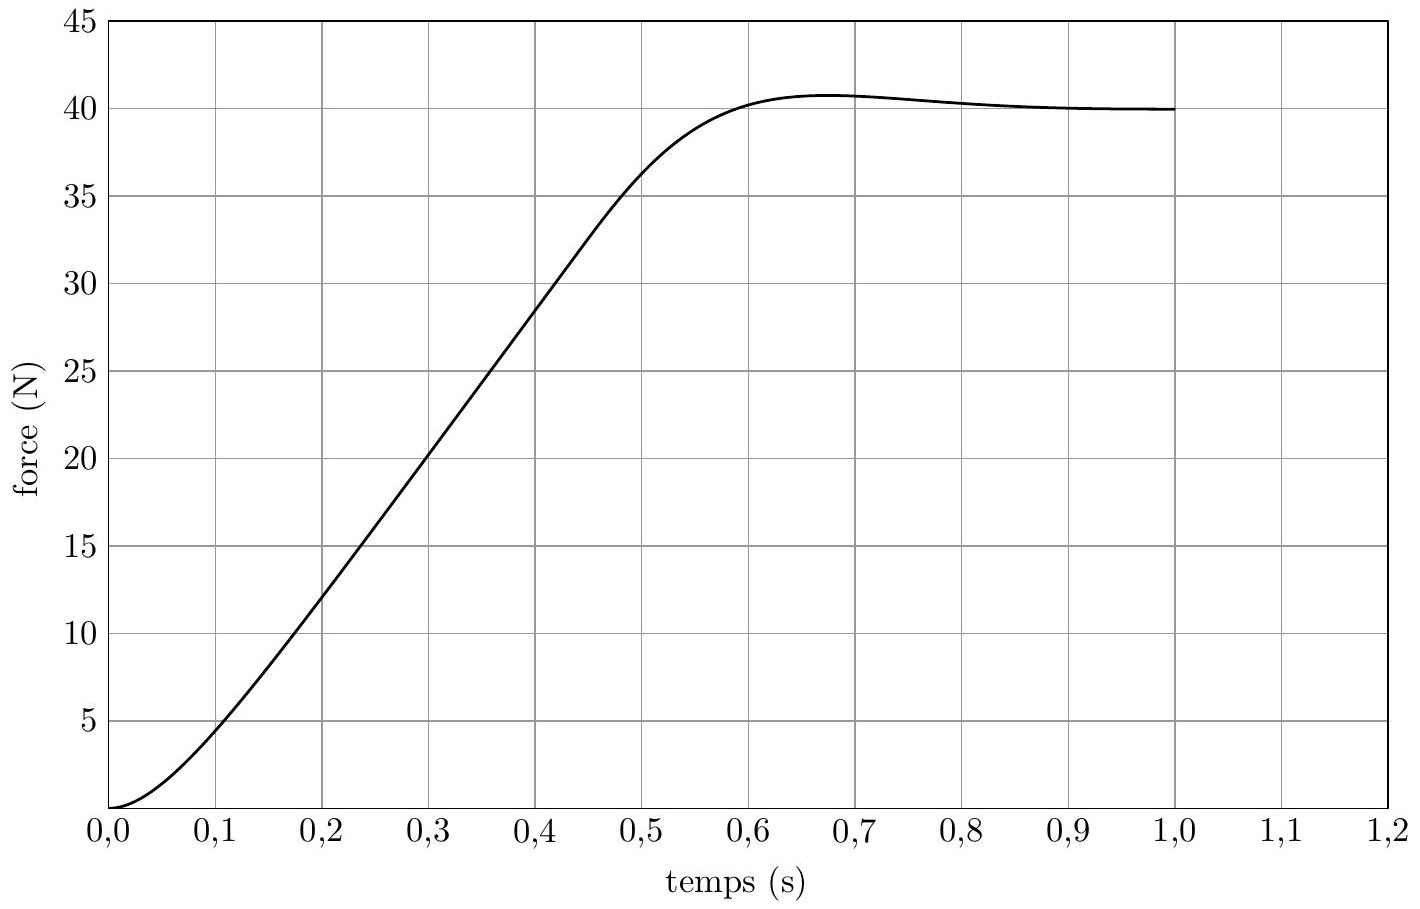
\includegraphics[width=\textwidth]{2025_09_16_5f2d7643f7e649c6833dg-14}
%%\captionsetup{labelformat=empty}
%%\caption{Figure 21 Réponse temporelle du modèle de connaissance pour une consigne de 40 N avec correction proportionnelle et limitation de la vitesse angulaire}
%%\end{center}
%%\end{figure}
%
%\begin{figure}[!h]
%\centering
%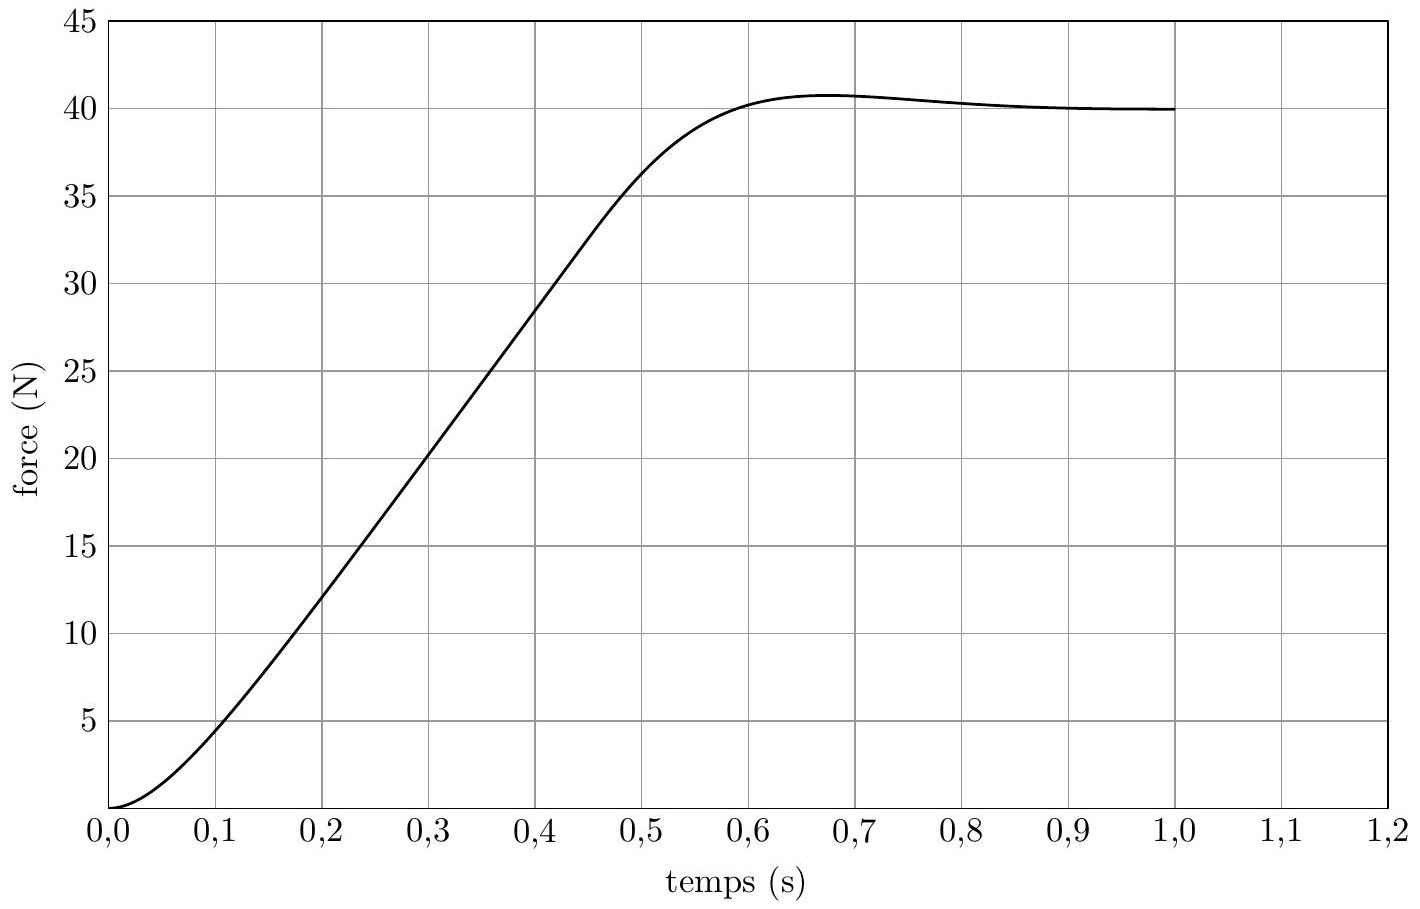
\includegraphics[width=.7\textwidth]{2025_09_16_5f2d7643f7e649c6833dg-14}
%\caption{\label{ccs_mp_2023_fig_21}  Réponse temporelle du modèle de connaissance pour une consigne de 40 N avec correction proportionnelle et limitation de la vitesse angulaire}
%\end{figure}
%
%
%
%%Q 28. 
%\question{\label{ccs_mp_2023_q_28}
%Conclure sur la capacité du correcteur proportionnel avec limitation de la vitesse angulaire à respecter le cahier des charges, en analysant l'écart entre les performances simulées (figure \ref{ccs_mp_2023_fig_21}) et les performances attendues. Se limiter aux critères pertinents du tableau \ref{ccs_mp_2023_tab_05}.}
%\ifprof
%\begin{corrige}
%\end{corrige}
%\else
%\fi
%


